\documentclass[twoside, 11pt]{epstfg}

\usepackage{lipsum}
\usepackage[numbers]{natbib}
\usepackage{fancysprefs}
\usepackage{booktabs}
\usepackage{wrapfig}
\usepackage{enumitem}
\usepackage{xfrac}
\usepackage{multirow}
\usepackage{subfigure}
\usepackage{listings}
\usepackage{colortbl}
\usepackage{graphicx}
\usepackage{epsfig}
\usepackage{xcolor}
\usepackage{hyperref}




\usepackage{tikz}

\usetikzlibrary{arrows}
\usetikzlibrary{patterns}
\usetikzlibrary{intersections}
\usetikzlibrary{calc}
\usetikzlibrary{fadings}

\definecolor{palette1}{HTML}{1B9E77}
\definecolor{palette2}{HTML}{D95F02}
\definecolor{palette3}{HTML}{7570B3}
\definecolor{palette4}{HTML}{E7298A}
\definecolor{palette5}{HTML}{66A61E}
\definecolor{palette6}{HTML}{E6AB02}
\definecolor{palette7}{HTML}{A6761D}
\definecolor{palette8}{HTML}{666666}
\definecolor{lightgray}{gray}{0.8}
\definecolor{verde}{RGB}{0,5,1}

\newcolumntype{g}{>{\columncolor{lightgray}}l}

\tikzstyle{vnlin}=[rectangle, inner sep=0pt, minimum height=6pt, minimum width=0pt, draw, fill=black]
\tikzstyle{hnlin}=[rectangle, inner sep=0pt, minimum height=0pt, minimum width=6pt, draw, fill=black]
\tikzset{>=latex}

\bibliographystyle{abbrv}

\title[spa]{Un enfoque de robótica virtual para personas que tienen discapacidad motora}
\title[eng]{A virtual robotic approach for people with motor disabilities}
\author{Cristina Kasner Tourné}
\tutor{Francisco de Borja Rodriguez Ortiz}
\date[spa]{Enero 2017}
\date[eng]{Enero 2017}

\setdegreeDouble

\begin{abstract}[spa]
	
La fusión de la Realidad Virtual con la robótica supone una apertura a infinitas posibilidades. 

Ambas tecnologías están en continuo desarrollo, de hecho la realidad virtual empezó a darse a conocer muy recientemente, a pesar de que su nacimiento data sobre  (año).

En los últimos años estamos presenciando cómo la Realidad Virtual va haciéndose un hueco en las tecnologías que usamos habitualmente. Quizá el uso más comercial que se le está dando es en lo referente al mundo de los videojuegos.
Sin embargo se puede aplicar a muchos otros campos , en concreto al campo de la salud , donde se están obteniendo muy buenos resultados (en cirugía, rehabilitación, etc).

Este trabajo pretende explorar el uso de la Realidad Virtual y la robótica como herramienta enfocada a personas con movilidad reducida , ayudarles a ser más independientes y dándoles la posibilidad de transportarse de forma virtual por entornos reales.

Para conseguir este objetivo se ha construido un sistema que consta de un \textbf{robot} y las \textbf{Oculus Rift} (gafas de realidad virtual).
El robot se controla desde las Oculus Rift, de forma que si el usuario lleva puestas las gafas, podrá controlar el robot con movimientos de cabeza.
El usuario verá a través de las gafas todo lo que vea el robot, actuando éste último como extensión de la vista del usuario.

Además hemos diseñado el proyecto de forma que la conexión entre el robot y las gafas sea a través de red inalámbrica, lo que le da al robot una libertad de movimiento fundamental para el objetivo que se persigue.

A lo largo del desarrollo del trabajo han surgido varias complicaciones, la gran mayoría referentes a la utilización de los sensores de las Oculus y de la librería de las mismas, que aún no está perfectamente adaptada a la versión DK2 de las gafas.

Esto se ha ido solucionando calibrando el movimiento de los servomotores mediante pruebas experimentales.

Una vez que se terminó de construir el robot e implementar el sowftware, se realizaron pruebas con diferentes usuarios para valorar su usabilidad.
Los resultados de las primeras pruebas no fueron muy positivos ya que el sistema de control que se había implementado era poco intuitivo y al usuario le costaba mucho manejar el robot.

En base a las primeras pruebas se ideó una nueva interfaz de control que dió mucho mejores resultados. Se ve cómo al principio de estas segundas pruebas a los usuarios les resulta bastante complicado controlar con precisión los movimientos del robot, ya que no están acostumbrados a moverse en base a los movimientos de la cabeza.Por ello al final de estas pruebas se ajustó la velocidad de los servomotores para que el robot se moviera un poco más lento.

Una vez terminados todos los cambios se realizaron unas últimas pruebas a otros usuarios distintos. Los resultados son muy satisfactorios ya que queda reflejado cómo en pocos minutos la sensación de control de los usuarios aumenta y les cuesta mucho menos alcanzar los objetivos propuestos.

A pesar de las últimas valoraciones positivas, no es recomendable utilizar las gafas durante mucho tiempo seguido si el usuario no está acostumbrado a ellas ya que en algunos casos puede causar mareos.

El resultado final del trabajo es un dispositivo inalámbrico que el usuario puede manejar sólo con la cabeza y que le permite visualizar su entorno a través de las Oculus Rift.
Al utilizar las Oculus Rift dejamos abierta la posibilidad de ver, no solo el entorno en el que se mueve el robot, sino un entorno virtual creado por el propio usuario. Esta parte se deja como tema de estudio para trabajos futuros.

\end{abstract}

\begin{abstract}[eng] 
	The fusion of the virtual reality with Robotic involves an opening to infinite possibilities.
	
	Both technologies are in continuous development, indeed virtual reality began to be known very recently, while their birth dates (year).
	
	In the last years virtual reality is making a place for itself in the current technologies. Perhaps the more commercial use that is being given is in relation to video games. 
	However it is possible to  apply to many others fields, in particular to the field of health, where virtual reality is getting really good results (in surgery, rehabilitation, etc). 
	
	This work aims to explore the use of virtual reality and  Robotic as a tool focused to people with motor disabilities, help them to be more independent and giving them the possibility of transport themselfs into real environments using virtual reality tools. 
	
	For this purpose a system that consists on a \textbf{robot} and the \textbf{Oculus Rift} (glasses of reality virtual) has been built .
	The robot is controlled from the Oculus Rift, so while the user is wearing the glasses, the user can control the robot with head movements.
	The user will see through the glasses everything that the robot is seeing, so the robot acts like an extension of the user's view.
	
	Also the robot and the glasses are connected via wireless network , so the robot is free for move everywhere the user wants. This is essential for the objective that this work pursues.
	
	Along the development of the work several complications have emerged , the great most relating to the use the Oculus's sensors and to the library which is used for take information from the Oculus's sensors.
	
	This problems have been solving by the calibration of the servo-motor by experimental tests.
	
	Once the robot was built and the sowftware was implemented, differente users did some test for rating the usability of the project.
	The results of the first tests were not positive due to the control system which was implemented was not intuitive and it was very difficult for the user to control the robot.
	
	Based on the results of the first tests it was designed a new control system. This new system has shown much better results than the first tests . At the beginning of these second tests it was quite complicated for the users to control the movements of the robot, since they are not used to move based on the movements of the head. That is the reason why at the end of these tests ,servomotors speed was adjusted with the objective of making the robot slower.
	
	 After all the changes were completed, a few final tests were made to other users. The results were very satisfactory since them reflected how in a few minutes the feeling of control of the users increases. Also it was easier for the users achieve the proposed goals.
	 
	 Despite the latest ratings positive, it is not recommended to use the glasses during much time without stop because the user can suffer dizziness.
	 
	 The final result of the work is a wireless device that the user can control only with the head. The devices  allows  the user to view himself environment through the Oculus Rift. Use Oculus Rift give the chance to see, not only the environment where the robot is , but a virtual environment created by the user. This part is left as subject of study for future work.
\end{abstract}

%\keywords[spa]{}
%\keywords[eng]{}

\newglossaryentry{cpd}{
	name = {CPD},
	longplural = {Centros de Proceso de Datos},
	description = {Centro de Proceso de Datos}
}

\newglossaryentry{nic}{
	name = {NIC},
	description = {Tarjeta de Interfaz de Red}
}

\newglossaryentry{irq}{
	name = {IRQ},
	description = {Petición de interrupción}
}

\newglossaryentry{api}{
	name = {API},
	description = {\textit{Application Programming Interface}}
}

\newglossaryentry{SPAN}{
	name = {SPAN},
	description = {\textit{Switched Port ANalyzer}}
}

\newglossaryentry{BPF}{
	name = {BPF},
	description = {\textit{Berkeley Packet Filter}, \cite{mccanne1993bsd}}
}

\newglossaryentry{NAPI}{
	name = {NAPI},
	description = {``New API'', una API de Linux desarrollada para mitigar interrupciones en \textit{drivers} de red y mejorar el rendimiento bajo condiciones de alta carga}}

\newglossaryentry{driver}{
	name = {Driver},
	text ={\textit{driver}},
	description = {Controlador de dispositivo: un programa que permite al sistema operativo interactuar con un periférico hardware}}

\newglossaryentry{DMA}{
	name = {DMA},
	description = {\textit{Direct Memory Accesss}, un sistema que permite a los periféricos acceder directamente a la memoria del sistema}
}

\newglossaryentry{padding}{
	name = {Padding},
	text = {\textit{padding}},
	description = {Datos ``de relleno'' que se añaden a una estructura de datos para alinearla a un tamaño concreto}
}

\newglossaryentry{RAID}{
	name = {RAID},
	description = {\textit{Redundant Array of Independent Disks}, una tecnología de virtualización de almacenamiento de datos que combina múltiples discos en una única unidad virtual, mejorando rendimiento y/o redundancia}
}

\newglossaryentry{RSS}{
	name = {RSS},
	description = {\textit{Receive Side Scaling}, una tecnología para \textit{drivers} de red que permite distribuir de forma eficiente los paquetes recibidos entre varias CPUs}
}

\newglossaryentry{RoCE}{
	name = {RoCE},
	description = {\textit{RDMA over Converged Ethernet}, tecnología de Mellanox para permitir acceso directo a memoria remota (RDMA) a través de redes Ethernet}
}

\newglossaryentry{NUMA}{
	name = {NUMA},
	description = {\textit{Non Uniform Memory Architecture}, diseño de sistemas multiprocesador con memoria local para cada procesador.}
}

\begin{document}

\selectlanguage{spanish}

\frontmatter

\maketitle[spa]
% \maketitle[eng]

\makeinnertitle[spa]
% \makeinnertitle[eng]

\makeabstract[spa]
\makeabstract[eng]

\tableofcontents
\clearpage
\listoftables
\clearpage
\listoffigures
\cleardoublepage

\printnoidxglossaries

\mainmatter
\chapter{Introducción} 


\section{Motivación del proyecto}

Este proyecto busca explorar las posibilidades que nos ofrece combinar la robótica con la realidad virtual. En concreto pretende estudiar la capacidad que la fusión de estas tecnologías tiene para incrementar la autonomía e independencia de personas con discapacidad motora.

Se ha investigado qué proyectos anteriores combinan robótica y realidad virtual y se han encontrado un gran número de ellos, muchos con resultados exitosos, como ya se explicará en el estado del arte. A pesar de que algún proyecto anterior ya estaba enfocado al tema de la discapacidad, la gran mayoría se centran en intentar estimular a estas personas y no en tratar de hacer que su entorno sea más accesible.

Una de las ventajas de hacer un proyecto basado en robótica y realidad virtual es que ambas tecnologías tienen un gran potencial.
El campo de la \textbf{robótica} lleva muchos años en desarrollo y mejora exponencialmente a lo largo del tiempo. Está inmerso en nuestro día a día y no paramos de sorprendernos con nuevos avances como las impresoras 3D, los drones o los brazos mecánicos.
Por otra parte puede parecer que la \textbf{realidad virtual} es una tecnología muy reciente pero lo cierto es que  lleva mucho tiempo estudiándose. En 1968 Ivan Sutherlan creó el primer casco de realidad virtual pero, como se explicará más adelante, aún no tenían las herramientas necesarias para desarrollar proyectos de realidad virtual de calidad.

Ahora nos encontramos en un momento en el que ya podemos empezar a disfrutar de la realidad virtual. Tenemos las CardBoard, las Oculus Rift, etc, a nuestro alcance.
El uso más generalizado que se está dando a estas herramientas es en el mundo de los videojuegos.
Viendo el potencial que tiene unir ambas tecnologías, resulta muy interesante explorar nuevas aplicaciones, en esta ocasión orientadas a mejorar la calidad de vida de un amplio sector de la sociedad.


La realidad virtual nos ofrece la posibilidad de \textbf{crear un entorno} en el cual, con el software adecuado, el usuario puede \textbf{interactuar} con otros usuarios, participar en actividades de \textbf{ocio y entretenimiento}, etc, sin necesidad de moverse de casa.
Además puede resultar muy interesante utilizar esta tecnología para \textbf{reproducir virtualmente entornos reales} a los que el usuario tenga difícil acceso.

El primer paso para conseguir esto es introducir imágenes del entorno en tiempo real dentro del mundo virtual. Para ello debemos disponer de un mecanismo móvil(p.ejemplo: un robot) que sea capaz de capturar fotogramas y mandárselas al usuario.  
Para que el usuario pueda ver dichas imágenes se utilizarán las Oculus Rift, unas potentes gafas de realidad virtual que son capaces de crear una \textbf{sensación de inmersión} total en cualquier entorno.
Ya que este trabajo está orientado a personas con movilidad reducida sería ideal que se pudiera controlar el movimiento del robot y de la cámara solo con el movimiento de la cabeza. En un futuro, no sería difícil adaptar este control a través de mandos.

¿Porqué utilizar las Oculus Rift?  Al ser las Oculus gafas de realidad virtual,si consiguiéramos una correcta conexión entre las gafas y el robot, se nos abrirían muchísimas posibilidades. Se podría modificar el entorno según las necesidades del usuario, integrar realidad aumentada para controlar una casa domotizada, incluir en el mundo virtual más entornos, a parte del real, donde el usuario pueda interactuar, realizar actividades de ocio, etc.
De esta forma daríamos al usuario más independencia y le abriríamos un mundo al que hasta ahora, tiene difícil acceso.

\section{Objetivos}\label{Objetivos}
El objetivo de este proyecto consiste en diseñar un dispositivo que actúe como extensión de la vista del usuario a través de una webcam implantada en el robot. El usuario deberá ser capaz de controlar la cámara con tan solo el movimiento de la cabeza, ya que el proyecto está orientado a personas con movilidad reducida.
Las imágenes se reproducirán a través de unas gafas de realidad virtual: las Oculus Rift. Esto nos permitiría, en un proyecto futuro, añadir realidad virtual o aumentada a las imágenes que captura la cámara.

Para ello definimos pequeños objetivos que debemos ir implementando para conseguir la meta final: streaming, movimiento de la cámara y visualización del entorno.

\subsection{Streaming}
Como se ha explicado anteriormente, debemos ser capaces de ver en las Oculus Rift a tiempo real todo lo que capta la cámara.

Dado que la comunicación con las Oculus Rift debe ser a través del PC al que estén conectadas , el streaming deberá \textbf{transmitirse desde la cámara hasta el PC}.

Por lo tanto uno de los primeros objetivos es implementar un método de comunicación a través del cual se puedan conectar  la cámara y el PC. Además se deberá implementar un software que capture la salida de la webcam y transmita el vídeo a tiempo real, es decir, que el usuario pueda saber con la mayor exactidud posible, el entorno que rodea al robot en todo momento. Por último se necesita un software que recoja el video en el PC.

\subsection{Movimiento de la cámara}
Otro de los objetivos básicos es que el usuario sea capaz de controlar la dirección y posición de la cámara con el movimiento de la cabeza. Para ello dotaremos a la cámara de un soporte móvil, un robot, que se explicará en el capítulo de Análisis.

Para controlar la cámara definimos dos fases del movimiento:
\begin{itemize}
	\item \textbf{Fase de exploración:}
	Durante la exploración la cámara no se mueve de sitio, tan solo explora el entorno.
	Los movimientos que se han decidido implementar para esta fase serán:
	\begin{itemize}
		\item Movimiento vertical : El usuario podrá mirar hacia arriba y hacia abajo.
		\item Movimiento horizontal : La cámara deberá ser capaz de rotar sobre si misma permitiendo al usuario mirar hacia ambos lados.
	\end{itemize}
	\item \textbf{Fase de transporte:}
	El usuario, enviando los comandos pertinentes al robot, podrá llevar la cámara a cualquier punto de la habitación.
	
\end{itemize}

Para este objetivo, el diseño tendrá un papel esencial ya que el control del robot debe ser sencillo e intuitivo. Se intentará crear un sistema de control con la cabeza que no sea complicado para el usuario.

\subsection{Visualización del entorno}
El último de los objetivos que es necesario desarrollar para el proyecto es conseguir visualizar en las Oculus Rift, el entorno en el que se encuentra la cámara.
Para ello necesitaremos un software que, en tiempo real, recoja el vídeo del PC y lo reproduzca en las gafas. 

A continuación se añade un esquema a modo de resumen de los objetivos ya explicados.

\begin{figure}[h!]
	\centerline{
		\mbox{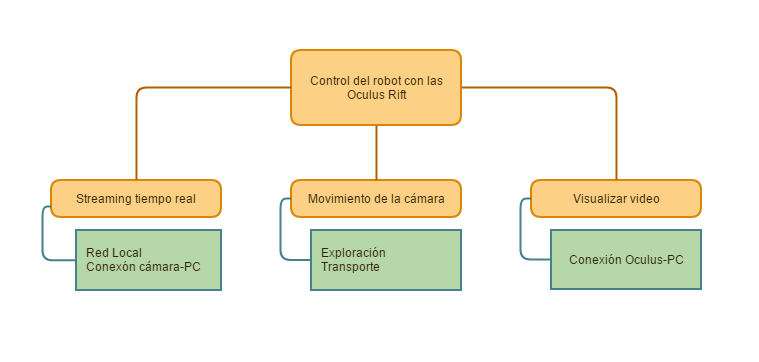
\includegraphics[width=7.00in]{images/objetivos.png}}
	}
	\caption{Resumen de los objetivos del proyecto}
\end{figure}


\newpage
\section{Desarrollo y plan de trabajo}

El desarrollo de este proyecto de fin de grado se puede dividir en tres fases:
\begin{itemize}
	\item \textbf{Investigación y aprendizaje:} Durante esta primera fase me documenté acerca de la realidad virtual, de sus aplicaciones y de las herramientas herramientas de las que disponía para realizar el trabajo. También busqué proyectos parecidos que unieran la robótica y la realidad virtual para saber que placas funcionaban mejor con gafas de realidad virtual.
	
	\item \textbf{Diseño y desarrollo:} Una vez adquirida la base de conocimiento necesaria para empezar el proyecto pude empezar la fase dos, que incluye:
	\begin{itemize}
		\item Diseño y construcción del robot
		\item Diseño e implementación del software
	\end{itemize}

	\item \textbf{Pruebas:} Durante la fase de pruebas un grupo de usuarios utilizó y valoró el proyecto. Además se hicieron cambios de diseño en base a la valoración de los usuarios .
\end{itemize}

\begin{figure}[H]
	\centerline{
		\mbox{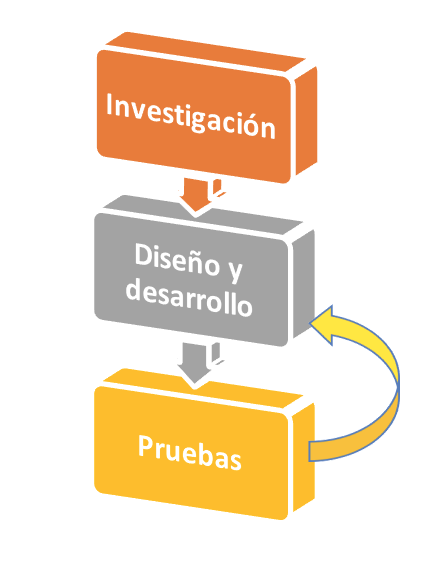
\includegraphics[width=2.50in]{images/Plan.png}}
	}
	\caption{En este grafo queda resumido el plan de trabajo. Se puede ver cómo la fase de pruebas vuelve a la fase de diseño y desarrollo, ya que el proyecto va mejorando en base a lo que demandan los usuarios.}
\end{figure}
\newpage
\section{Estructura del documento}


El objetivo de este documento es explicar el trabajo realizado y los resultados obtenidos.

En el siguiente capítulo se explica el estado del arte, hablando brevemente de la realidad virtual y de algunos proyectos previos que utilizaban esta tecnología. Como se verá más adelante el capítulo se centra especialmente en proyectos relativos a salud y robótica.

Luego se verá el análisis, diseño y desarrollo del proyecto.

En el análisis se presentan los requisitos que debe cumplir nuestro sistema. Posteriormente se hace un estudio de diseño de los componentes del trabajo (robot, conexiones entre dispositivos...) y por último se explicará como se ha desarrollado el proyecto.

Los resultados y las pruebas realizadas para ver si el proyecto cumplía con el objetivo se verán en el capítulo "Pruebas y resultados" de este documento.

Para finalizar expondremos brevemente las conclusiones y el trabajo futuro que se puede realiza en base a este proyecto.

\chapter{Estado del arte}


En este capítulo se contará brevemente la historia de la realidad virtual.
También se presentarán diferentes proyectos que han utilizado la combinación de realidad virtual y robótica y cuales fueron sus resultados.

La cara más visible de esta tecnología es el uso que se le da en los videojuegos, no es su única aplicación. Los proyectos que aquí se exponen están más orientados a la salud o al control de dispositivos, ya que son más afines con este trabajo fin de grado.
Los proyectos relativos al campo de la salud, se aplican mayoritariamente a rehabilitaciones. Esto es muy interesante para este trabajo ya que muestra cómo usuarios con alguna dificultad motora responden bien a entornos virtuales.
También se hablará de cómo se están integrando actualmente  las dos tecnologías que utilizaremos en este trabajo: la robótica y la realidad virtual.

La explicación de estos proyectos en este capítulo pretende dar una fotografía general del estado y las aplicaciones actuales de ambas tecnologías, dando especial importancia a aquellos proyectos con un enfoque similar al de nuestro trabajo.

\section{Evolución histórica de la realidad virtual}
La realidad virtual comenzó siendo ciencia ficción y poco a poco está ganando terreno en la vida cotidiana, ya sea en el mundo de los videojuegos, la medicina o la aviación, entre otros campos.

A pesar de ser una tecnología de la que se ha empezado a hablar hace relativamente poco, los primeros proyectos que utilizaban realidad virtual datan de los años 60.

Uno de los  acontecimientos más significativos del inicio de la realidad virtual es la creación de \textbf{“The Sword of Damocles”} , un casco de realidad virtual (HMD- head-mounted display)  creado por Ivan Sutherland en 1968 \cite{Sutherland}.

The Sword of Damocles permitía ver las imágenes tridimensionales generadas por el
ordenador superpuestas ópticamente, a través de un prisma, al entorno real que rodeaba al usuario.

 El sistema estaba montado sobre un brazo mecánico suspendido del techo que también servía para detectar, mediante el uso de sensores, la posición y la orientación de la cabeza del usuario. De este modo, cuando el usuario se movía, los objetos creados por el ordenador daban la impresión de encontrarse en una posición estable dentro del entorno real.

Es lógico preguntarse cómo ha tardado tanto en llegar al mercado la realidad virtual si ya en 1968 consiguieron sacar adelante este proyecto.

La respuesta es que \textbf{la tecnología de los años 60 aún no estaba preparada} para desarrollar herramientas de realidad virtual.

Para conseguir capturar la posición y el movimiento de la cabeza del usuario, se requería un brazo de \textbf{grandes dimensiones}.
Además la realidad virtual necesita una \textbf{capacidad de cómputo muy potente}. Problemas tales como "hidden line" solo podía ser resueltos con un ordenador que tenía la NASA en Houston, como especifica Sutherland en su trabajo \textit{A head-mounted three dimensional display} \cite{Sutherland}. 

\begin{figure}[h]
	\centerline{
		\mbox{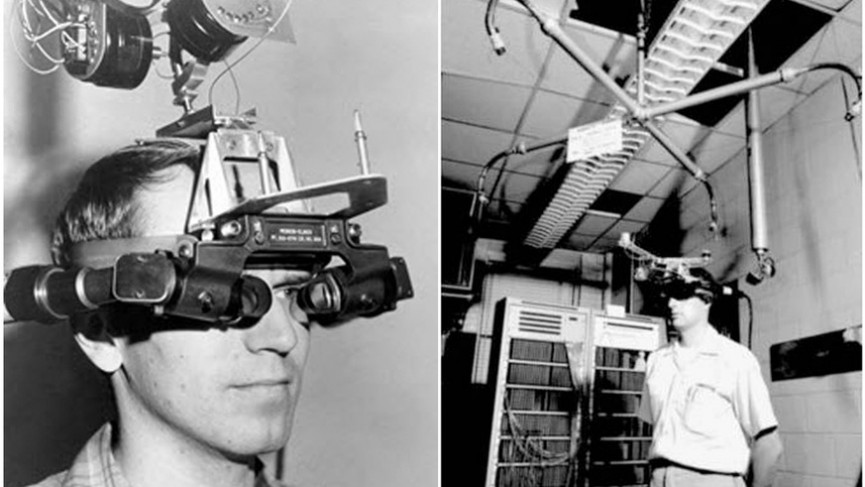
\includegraphics[width=.80\textwidth]{images/SwordOfDamocles.jpg}}
	}
	\caption{Sword of Damocles. Imagen obtenida de \textit{A head-mounted three dimensional display} \cite{Sutherland}}
	
\end{figure}


Al mismo tiempo Thomas A. Furness III empezó a introducir herramientas de \textbf{realidad virtual en entrenamientos de vuelo} \cite{kocian1977visually}, con el objetivo de que estos fueran mucho más seguros para los pilotos.
A pesar de que fue una gran aportación en este campo, la escasez de recursos y capacidad de cómputo también retrasaron mucho el desarrollo de estas herramientas.
 
Hoy en día tenemos la capacidad necesaria para desarrollar estas herramientas por lo que se siguen utilizando y mejorando ya que, no solo es más segura, sino que además es más barata.

Durante las últimas décadas del s.XX, se hicieron algunos proyectos de realidad virtual , pero no tuvieron mucho éxito debido a su alto coste.

Con el desarrollo exponencial que ha vivido la tecnología las últimas décadas, la realidad virtual ha ido haciéndose un hueco en la industria tecnológica.
El empujón definitivo vino con la creación de las \textbf{Oculus Rift}, en el año 2010.

\textbf{Palmer Luckey} es el fundador de Oculus VR (una compañía de realidad virtual) y el diseñador de la primera versión de las Oculus Rift.

Oculus Rift es un casco de realidad virtual (también nos podemos referir a ellas como gafas de realidad virtual) mucho más manejable que "The Sword of Damocles" , con mucha más calidad y con un coste asequible.
Uno de los grandes logros de Luckey con las Oculus Rift es que consiguió un ángulo de visión de 90º, algo nunca visto hasta el momento.

Tras el lanzamiento de las Oculus Rift, el mercado comenzó a interesarse por proyectos relacionados con la realidad virtual y a financiarlos.
Gracias a esto la tecnología ha podido desarrollarse y hoy podemos disfrutar de una realidad virtual con mucha más calidad y \textbf{sensación casi total de inmersión} en entornos virtuales.




\section{Realidad virtual y salud}
\label{sec:VR y salud}

La realidad virtual ofrece grandes posibilidades en el campo de la medicina. Permite estudiar cómo responde el paciente a distintos estímulos o cómo interactúa con diferentes entornos de forma bastante realista.

Podemos encontrar un ejemplo de esto en un proyecto que se realizó para evaluar el deterioro cognitivo en personas que sufren esclerosis múltiple. Para que dicha evaluación sea precisa se requiere de una gran cantidad de datos sobre la velocidad de procesamiento de la información, atención, etc. Esto se conseguía haciendo múltiples test que no siempre eran fieles a la realidad.
Ahora con la realidad virtual se consiguen crear entornos en los que el usuario tiene tal sensación de inmersión, que su \textbf{comportamiento es muy similar al que tendría en el entorno real}. Esto permite hacer un estudio mucho más amplio y realista de los estímulos del paciente y obtener resultados más completos.\cite{LamargueHamel201594}


Otra aplicación interesante es el uso de realidad virtual en programas de rehabilitación.
Se realizó un estudio a personas con hemiparesia, es decir, pacientes que han perdido parcial o totalmente la capacidad motora de las extremidades de uno de los lados de su cuerpo. El proyecto consistía en un software que mostraba por pantalla el movimiento de los pies  del usuario y le mandaba ejercicios para mejorar su locomoción. 
Los resultados de este estudio mostraron que la herramienta de realidad virtual era \textbf{efectiva para la rehabilitación de las capacidades motoras} de los pacientes y además es especialmente útil para aquellos que tienen dificultades para trasladarse hasta el hospital.\cite{Llorens2015418}

Los dos proyectos que se han presentado en este capítulo son ejemplos de cómo la realidad virtual ha contribuido a mejorar técnicas que ya se usaban anteriormente.

El siguiente proyecto también está enfocado a mejorar el tratamiento de pacientes pero, en esta ocasión, utiliza una característica propia de la realidad virtual, que es la inmersión en un entorno distinto al que se encuentra el paciente.

Esta capacidad que tiene la realidad virtual es muy útil para personas que se encuentran en un proceso de rehabilitación doloroso.

El experimento que se presenta a continuación se realizó con un paciente de 40 años con un 19\% de su cuerpo quemado. El trabajo consistía en utilizar un entorno virtual como paliativo durante los ejercicios de rehabilitación.
Se le proporcionó al paciente un casco de realidad virtual y se creó un entorno en el que el paciente pudiera "resguardarse" del dolor ocasionado por la rehabilitación.

\begin{figure}[h]
	\centerline{
		\mbox{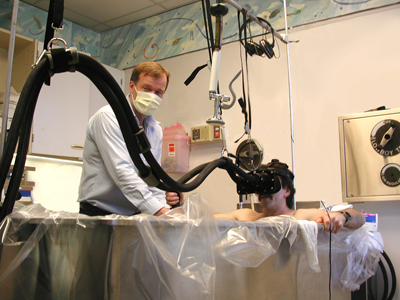
\includegraphics[width=.50\textwidth]{images/waterfriendly.png}}
	}
	\caption{Rehabilitación usando herramientas de realidad virtual. Imagen obtenida de \textit{Water-Friendly Virtual Reality Pain Control During Wound Care} \cite{JCLP:JCLP10244}}
	
\end{figure}

Los resultados fueron muy positivos. El usuario puntuó la sensación de dolor en un 7 sobre 10 cuando no usaba realidad virtual y en un 2 sobre 10 utilizando realidad virtual.\cite{JCLP:JCLP10244}

Estos experimentos suponen una prueba de la increíble \textbf{capacidad de inmersión} que nos proporciona la realidad virtual, aspecto muy importante para nuestro trabajo.


\section{Robótica y realidad virtual.} 
\label{sec:robotica y VR}

A continuación se presentan algunos proyectos de robótica que utilizan técnicas de realidad virtual. Es interesante ver, en los resultados de estos trabajos, cómo ambas tecnologías se complementan de forma muy beneficiosa.

Puesto que al final de este trabajo lo que se quiere conseguir es controlar un robot a través de una interfaz que utiliza realidad virtual, es interesante estudiar cómo ha resultado esto en proyectos parecidos.

En 1997 , el IMG (Intelligent Mechanisms Group) de la NASA y el instituto de robótica de la Carnegie Mellon University desarrollaron las \textbf{interfaces de control} necesarias para teledirigir a Nomad, un robot diseñado para la exploración de planetas. \cite{Nguyen2001}

Hasta el momento este control era altamente complicado, ya que requería del uso de muchos comandos poco intuitivos. Para mejorar y facilitar esto, crearon dos interfaces:\textit{ Virtual Dahsboard Interface} y \textit{Telepresence Interface}.

\textit{Virtual Dashboard interface} consiste en un panel de control donde el operador podía ver de forma simple el estado actual de Nomad y controlarlo de forma intuitiva.

\textit{Telepresence Interface} es una interfaz que hace uso de la cámara panorámica de Nomad. A través de dicha interfaz el usuario podía ver las imágenes capturadas por Nomad e incluso podía girar el punto de vista o ampliar la imagen para conocer mejor el entorno.

Estas imágenes se reproducían en una pantalla ancha, parecida a un parabrisas de un coche, frente al operador, para dar más sensación de telepresencia.

Uno de los inconvenientes de este trabajo fue el delay a la hora de recibir las imágenes (5 segundos), que hacía más difícil el control.
A pesar de esto \textbf{los resultados fueron positivos}, concluyendo que los operadores manejaban mejor el robot haciendo uso de la Telepresence Interface que sin ella.


Otra de las aplicaciones de la combinación de robótica con realidad virtual es la mejora en \textbf{intervenciones quirúrgicas}.
\begin{figure}[h]
	\centering
	\subfigure[]{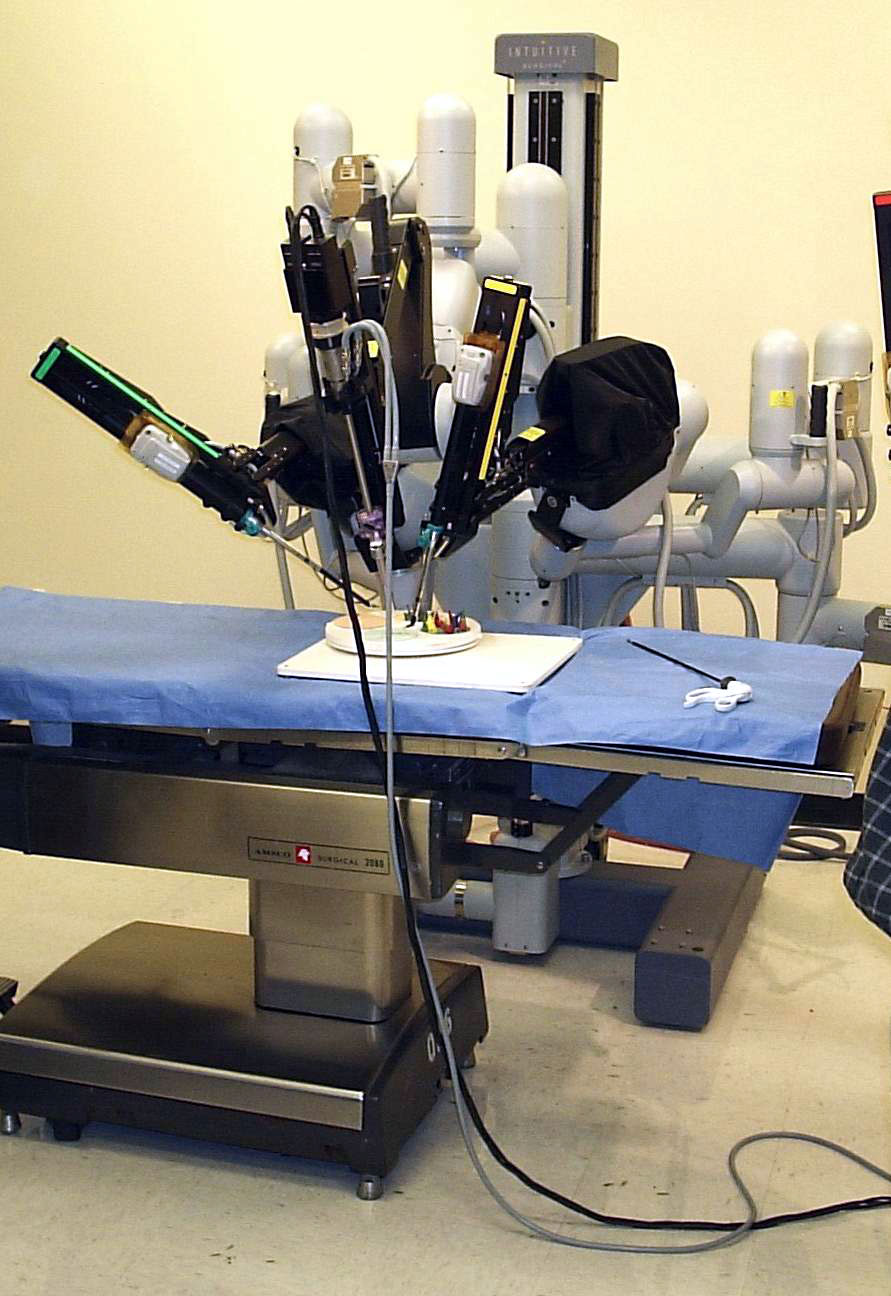
\includegraphics[width=51mm]{images/Laproscopic_Surgery_Robot.jpg}}
	\subfigure[]{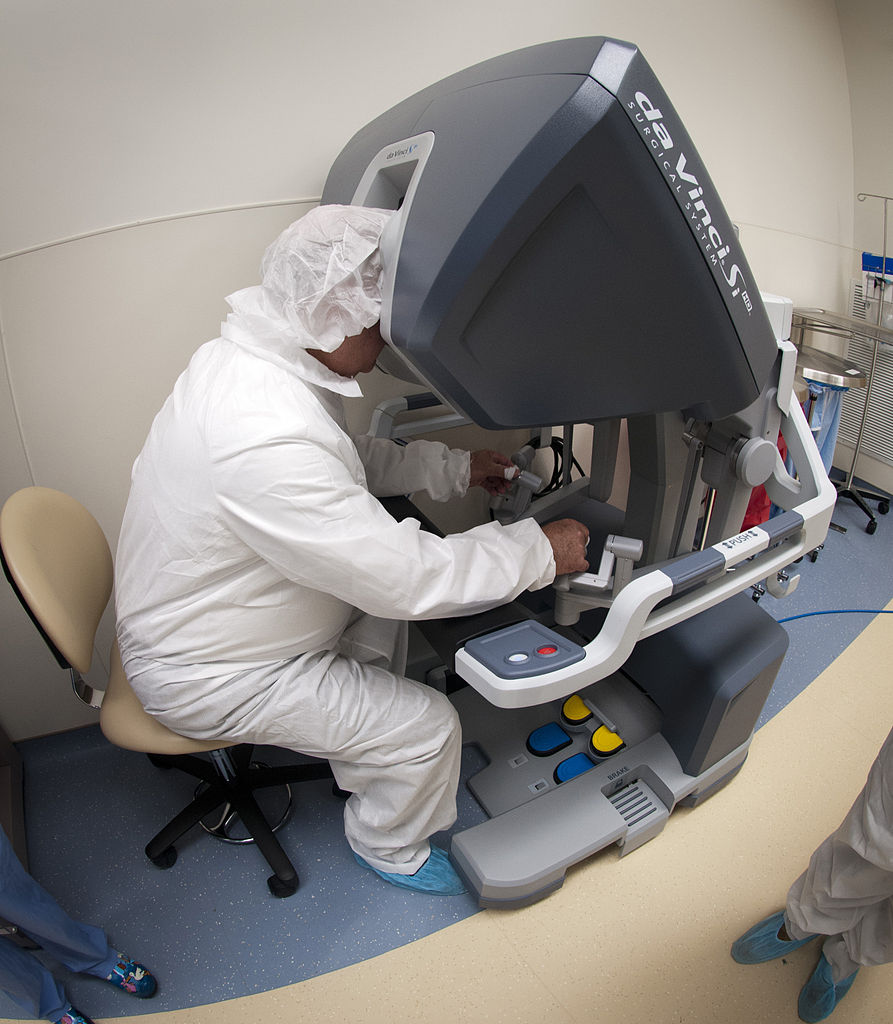
\includegraphics[width=65mm]{images/cirujano.jpg}}\\
	\caption{Da Vinci Surgical System} \label{daVinci}
\end{figure}


Un ejemplo de esto es \textbf{Da Vinci Surgical System}, un sistema en el cual el cirujano controla, a través de unos mandos, las herramientas necesarias para operar al paciente. Además tiene una pantalla 3D en la que se ve a tiempo real la zona que está siendo intervenida.
Este sistema hace posible que el cirujano realice \textbf{movimientos mucho más precisos}, además de facilitarle una postura más cómoda durante la operación. \cite{Hubens2003}

Lo que nos muestran los resultados de estos proyectos es que los usuarios son capaces de manejar dispositivos que ven a través de realidad virtual de forma exitosa. Esto también es imprescindible en nuestro trabajo ya que el usuario debe controlar el robot tan solo con las gafas de realidad virtual. 

%En educación hay varios programas de realidad virtual que hacen el aprendizaje más sencillo y completo a los estudiantes. Un ejemplo de esto es la visualización de brazos robóticos para diseñar correctamente el movimiento.
%Es relativamente complejo traducir cada movimiento de las articulaciones del brazo robótico en la posición finla de éste. Si estas pruebas se hicieran directamente sobre el robot, sería muy sencillo romperlo. Con los programas de realidad virtual se simulan todos los movimientos sin peligro de malgastar recursos. [ref]



\chapter{Análisis}
\label{chap:sistemadesarrollado}
Una vez conocido el estado actual de la robótica y la realidad virtual, el siguiente paso es analizar a fondo el proyecto que se quiere desarrollar.
Para ello se deben definir los requisitos que debe cumplir el trabajo, basando estos requisitos en los objetivos propuestos en la sección de \textit{Objetivos} \ref{Objetivos}. De esta forma el trabajo queda dividido en pequeñas tareas y facilita su implementación.

En el capítulo de \textit{Objetivos} \ref{Objetivos} se explica que la meta final del proyecto es conseguir que el usuario pueda controlar una cámara con el movimiento de cabeza y ver todo lo que la cámara vea.
La forma más eficiente de hacer que la cámara sea móvil es construir un robot con ruedas que lleve la cámara integrada. 

De esta forma cuando el usuario mueva la cabeza, se le enviarán las instrucciones necesarias al robot para que se mueva. A su vez el robot le estará mandando video a tiempo real al usuario, que lo verá a través de las Oculus Rift.


El proyecto por lo tanto se divide en 3 problemas:
\begin{enumerate}
	\item \textbf{Construcción del robot} $\rightarrow$ para ello necesitaremos una placa base, una cámara y la estructura que le permita desplazarse.
	\item \textbf{Streaming}$\rightarrow$ Debemos conseguir transmitir a tiempo real todo lo que ve el robot a la Oculus
	\item \textbf{Control del robot}$\rightarrow$ Queremos que el robot sea una extensión de los sentidos del usuario, por lo que debemos idear movimientos intuitivos para que el usuario mande comandos de movimiento al robot.
\end{enumerate}

Vamos a desarrollar cada uno de ellos, identificando qué funcionalidades básicas debe cumplir.

\section{Requisitos Funcionales}

\subsection{Construcción del Robot}


El robot debe ser un dispositivo fácil de controlar , que a su vez actúe como una extensión de los ojos del usuario, dándole a éste la sensación de inmersión un espacio real.
Por tanto los requisitos que debe cumplir el robot son los siguientes:


\begin{itemize}
	\item \textbf{RF-CR1: Grabar video y transmitirlo a tiempo real.}
	
	 Ya que el robot va a actuar como sentido de la vista del usuario, debe enviar de forma continua imágenes a tiempo real del entorno que le rodea.
	
	
	\item\textbf{RF-CR2: Desplazarse en todas las direcciones del plano.} 
	
	Uno de los posibles usos del trabajo es utilizar el robot como dispositivo de exploración del entorno. Para ello es necesario que el robot pueda moverse en todas las direcciones, como si del propio usuario se tratara.
	
	
	\item\textbf{RF-CR3: Recibir comandos de control a través de una red inalámbica.}
	
	Ya que un objetivo del proyecto es dar independecia al usuario el robot debe poder moverse por el espacio sin importar donde se encuentre el usuario. Esto se consigue diseñando un software de control que envíe los comandos de forma inalámbrica.
	
	
	\item\textbf{RF-CR4: La cámara debe apuntar en la misma dirección que la cabeza del usuario.} \label{RF-CR4} 
	
	La cámara del robot hará las funciones de los ojos del usuario, por lo tanto debe tener la misma orientación respecto al cuerpo del robot que la orientación de la cabeza respecto al cuerpo del usuario.
\end{itemize}



\subsection{Streaming}
Se quiere conseguir la máxima sensación de inmersión para la persona que controla el robot.
Para ello los requisitos principales que debe cumplir son:

\begin{itemize}
	\item\textbf{RF-S1: La transmisión de video debe ser  a tiempo real, con la mínima latencia posible.}
	
	Si las imágenes del entorno llegan al usuario con un desfase temporal importante respecto al movimiento de la cabeza, se reducirá la sensación de inmersión y será mucho más dificil controlar el robot.
	
	\item\textbf{RF-S2: Imagen desdoblada}
	
	El usuario verá el video con las Oculus Rift, por lo que la imagen debe estar desdoblada (formato SBS, que se eplicará en la sección de desarrollo).
	
	\item\textbf{RF-S3: Transmisión de video inalámbrica}
	
	Al igual que en el requisito \textbf{RF-CR3}, la transmisión del streaming también debe ser inalámbrica ya que, de otro modo, se perdería la libertad dde movimiento del robot.

	
	
\end{itemize}



\subsection{Control del Robot}

Como hemos dicho anteriormente, se pretende que la cámara, soportada por el robot, sea una extensión de los ojos de usuario.Por esto es lógico que se controle con el movimiento de cabeza de la persona que esté recibiendo el video.
Dentro del control del robot vamos a diferenciar entre control del movimiento del robot y control de la dirección de la cámara:

\begin{itemize}
	\item Movimiento del robot :
	
	\textbf{RF-CTRL1: El control del robot solo depende del movimiento de la cabeza del usuario}
	
	La interfaz de control del robot constará solo de movimientos de la cabeza del usuario ya que el trabajo está orientado a personas con discapacidad motora.
	\item  Movimiento de la cámara:
	
	\textbf{RF-CTRL2: La cámara debe moverse acorde con el movimiento de la cabeza del usuario.}
	
	Este requisito es necesario tanto para el control del robot como para la sensación de inmersión.
	\textit{Por ejemplo:} Es importante que si el usuario hace el movimiento de mirar hacia arriba, la imagen que le llegue sea acorde con el movimiento.
	
	
	
\end{itemize}


\section{Requisitos no funcionales}

\begin{itemize}
	\item \textbf{RNF1 - Usabilidad}
	
	
	El sistema para controlar el movimiento del robot y de la cámara debe ser intuitivo, sin requerir movimientos de cabeza inusuales por parte del usuario.
	
	
	
	\item \textbf{RNF2 - Accesibilidad}
	
	Dado que el trabajo está orientado a personas con discapacidad motora, el control del robot debe ser accesible para las mismas, de forma que no requiera de movimientos bruscos o exagerados. 
	
	\item \textbf{RNF3 - Sistema configurable}
	
	El sistema de movimiento y control del robot no debe ser cerradp, por el contrario debe contar con parámetros de configuración para poder adactar el sistema a las capacidades motoras de cada usuario.
\end{itemize}

\newpage
\chapter{Diseño}

Tras analizar los requisitos que debe cumplir el trabajo vamos a ver cómo se diseñará cada componente y como estarán integrados entre ellos.

Los componentes que forman el proyecto son: las gafas de realidad virtual Oculus Ridt DK2, un router(Xavi7968.), un ordenador \textcolor{red}{(ordenador)} y un dispositivo móvil con cámara integrada (robot).
El diseño de los componentes, el control del robot y las conexiones se realizaran en base a los recursos y herramientas disponibles, que también se presentarán en este capítulo.

Recordemos que el objetivo es construir un dispositivo que se comunique de forma inalámbrica con el usuario. El robot debe transmir imágenes a tiempo real del entorno y recibir comandos de movimiento para que el usuario pueda explorar el espacio.
Por lo tanto en términos generales, las tareas que desempeñarán los componentes son las siguientes:
\begin{itemize}
	\item \textbf{Robot} 
	
		Debe ser un dispositivo móvil, con una webcam integrada para poder transmitir imágenes.
		
		Además de la cámara el robot deberá tener integrado algún mecanismo de envío y recepción de datos.
	\item \textbf{Router}
	
		Se utilizará un router para crear un ared local a través de la cual se envíen tanto las imágenes como los comandos de control del robot.
	\item \textbf{Oculus Rift y PC}
		
		Las gafas de realidad virtual reproducirán las imágenes para el usuario. Deben estar conectadas a un PC que reciba el video y envíe los comandos al robot.
		
\end{itemize}


\section{Diseño del robot}

El robot que se utiliza en este proyecto está basado en un diseño anterior hecho por (Nombre del alumno que diseñó en robot). De este diseño hemos reutilizado (estructura???)

En un principio también se pretendía utilizar la misma placa: \textbf{Arduino Yun}.
Esta placa tiene la capacidad de conectarse a \textbf{internet a través de Wifi}, además tiene dos procesadores, el Atmega y el Atheros AR9331, lo que le permite de \textbf{combinar Arduino con Linux}. Esto era muy útil ya que el control de servomotores es muy sencillo con Arduino y tener un sistema operativo Linux en la placa nos permitía instalar programas de manejo de vídeo.
Tras muchas pruebas se decidió no utilizar esta placa ya que el módulo Wifi daba muchos problemas y se optó por utilizar la Raspberry Pi 3, de la que se hablará más adelante.

Finalmente el robot consta de:
\begin{itemize}
	\item Una placa base $\rightarrow$ Raspberry Pi 3.
	\item Dos ruedas conectadas con dos servos que permiten al robot desplazarse.
	\item Una cámara Logitech, conectada a la placa por USB.
	\item Un servo unido a la cámara.
	\item Una estructura de plástico impresa con la impresora 3D del Club de Robótica de la EPS.
\end{itemize}


A continuación se explicarán en detalle cada uno de los componentes del robot.

\subsection{Raspberry Pi 3 model B}
La Raspberry Pi 3 model B es un ordenador de placa reducida que lleva un sistema operativo Linux.
Su procesador es un ARM Cortex A53 de cuatro núcleos a 1.2GHz de 64 bits.
Tiene 1 GB de memoria RAM , 4 puerto USB, 40 pins GPIO, puerto HDMI , Ethernet y entrada para MicroSD.
Además tiene Wifi 802.11n integrado y bluetooth 4.1.

Tras rechazar el Arduino Yun como placa para el proyecto, la Raspberry Pi 3 quedó como mejor candidata ya que cumplía todos los requisitos necesarios. A saber:

\begin{itemize}
	\item \textbf{Módulo Wifi (802.11n Wireless LAN)}: Imprescindible para la transmisión.
	\item \textbf{S.O Linux}: Nos permite instalar programas de manejo y transmisión de video, como la librería mjpeg-streamer que se usará en este proyecto.
	\item \textbf{Puerto USB}: Para conectar la cámara y la fuente de alimentación.
	\item \textbf{GPIO}: Necesario para conectar los servomotores.
\end{itemize}


\begin{figure}[H]
	\centerline{
		\mbox{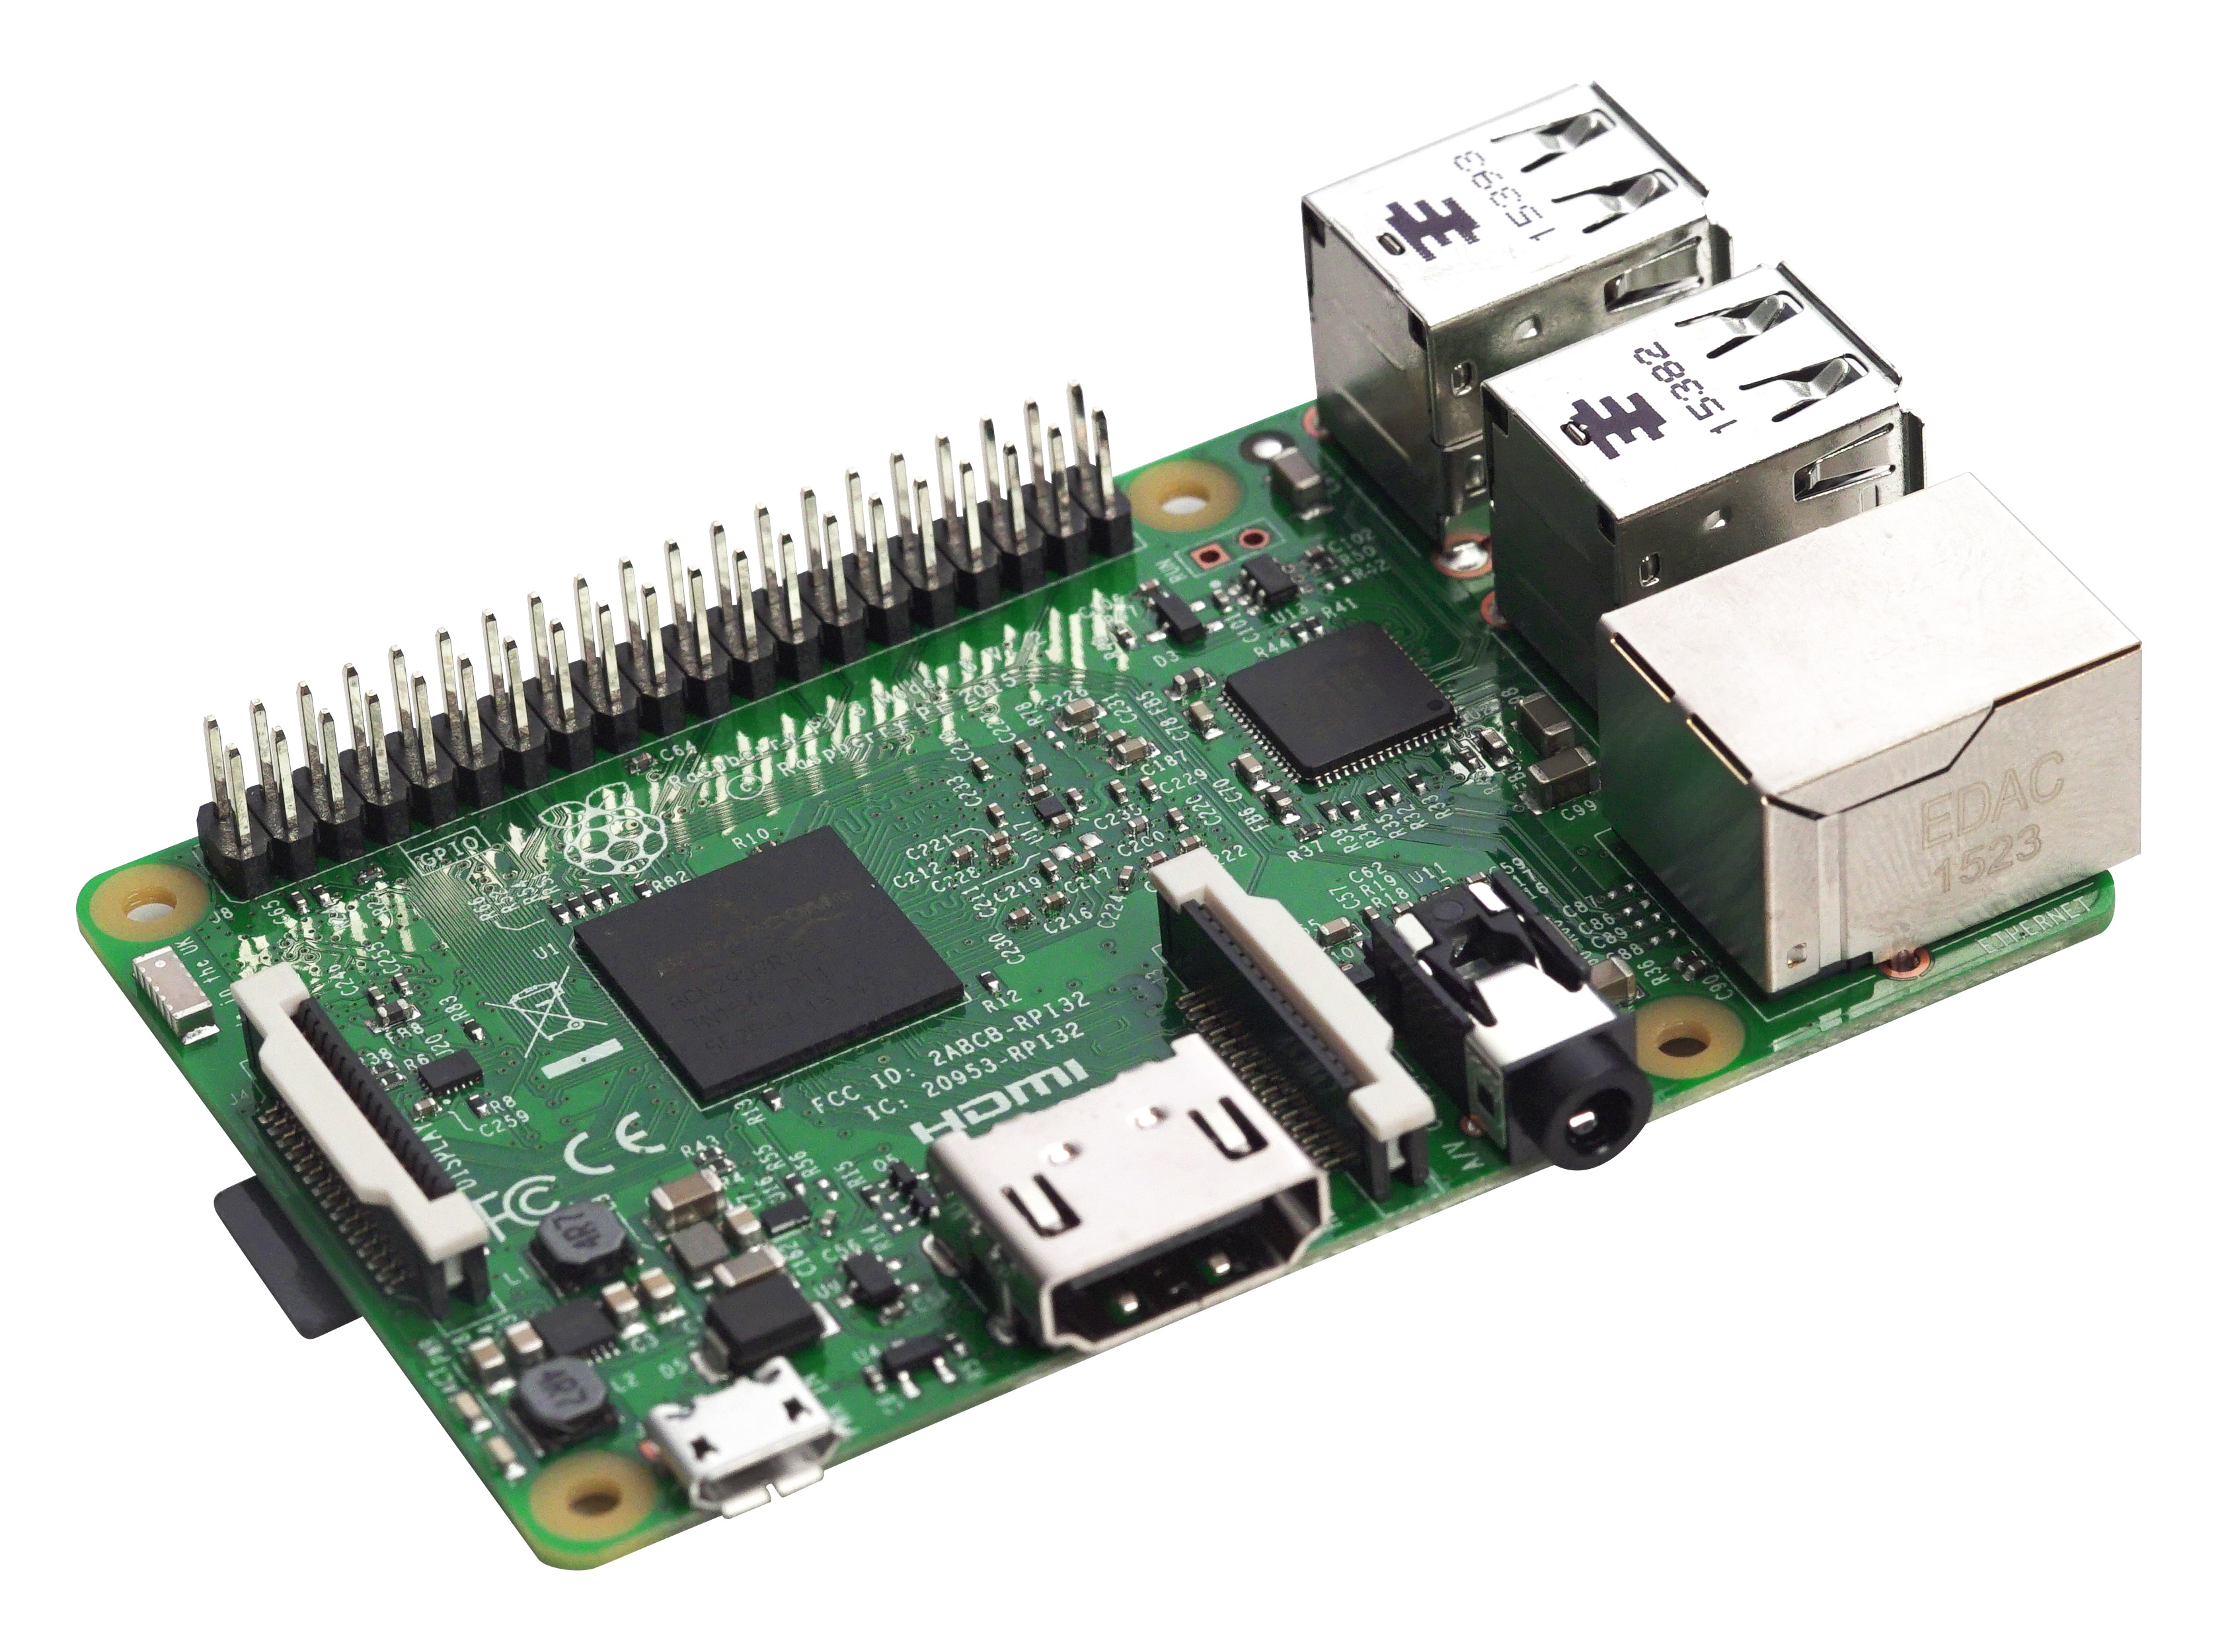
\includegraphics[width=.80\textwidth]{images/raspi3.jpg}}
	}
	\caption{Raspberry Pi 3 model B}
	
\end{figure}

\subsection{Servo motores}
El robot debe tener la capacidad de desplazarse, por lo que se diseñó con dos ruedas laterales que son controladas a través de dos servomotores de rotación continua. Otro requisito era que la cámara debía estar en todo momento orientada respecto al robot hacia la misma dirección que la cabeza del usuario está orientada respecto a su cuerpo \ref{RF-CR4}. Para poder cumplir este requisito se añadirá un servomotor al robot que esté unido a la cámara y pueda rotarla respecto al eje horizontal.

Antes de mostrar cómo se van a conectar los servomotores con las ruedas y la cámara y cómo reciben los comandos se va a explicar brevemente qué es un servomotor y cómo funciona:

Un servomotor es un dispositivo similar a un motor de corriente continua que tiene la capacidad de ubicarse en cualquier posición dentro de su rango de operación, y mantenerse estable en dicha posición. Una de las caráterísticas más importantes de estos dispositivos es que puede controlarse tanto en posición como en velocidad.


Los servos constan de:
\begin{itemize}
	\item Un motor de corriente continua
	\item Una caja reductora
	\item Un circuito de control
\end{itemize}

El sistema que utilizan los servomoters para controlar la velocidad y la posición de los motores de corriente continua es la modulación por anchura de pulso (PWM).

\paragraph{PWM}

Este sistema consiste en generar una onda cuadrada en la que se varía el tiempo que el pulso está a nivel alto, manteniendo el mismo período (normalmente), con el objetivo de modificar la posición según se desee.

\begin{figure}[h]
	\centerline{
		\mbox{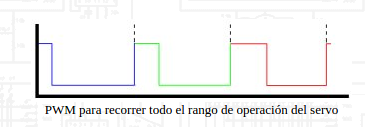
\includegraphics[width=.80\textwidth]{images/ondaServo.png}}
	}
	\caption{Onda cuadrada que representa los pulsos que se envían a los servomotores}
\end{figure}


Como hemos dicho, el control de la posición y la velocidad es un atributo característico de este tipo de motores y por tanto se va a explicar brevemente cómo funciona.\\
Para que un servo se mantenga en la misma posición durante un cierto tiempo, es necesario enviarle continuamente el pulso correspondiente.\\
El control de la velocidad se consigue alimentando el motor con una señal de pulsos con la frecuencia suficiente para que el motor no note las variaciones y haga un giro constante, ya que variando el porcentaje de tiempo de la señal rectangular en alta, y en baja, variamos la potencia que le entregamos al motor, con lo que podemos controlar la velocidad de giro.

En el robot utilizamos 3 servomotores.
Dos de ellos se utilizan para el movimiento de las ruedas y el tercero moverá la cámara permitiendo al usuario mirar hacia arriba y hacia abajo.
Los tres servos están controlados por el movimiento de la cabeza del usuario, que obtenemos gracias a las Oculus Rift.

\subsection{Cámara}

La cámara utilizada es una webcam USB. El proyecto también se podría haber hecho con una RaspiCam o con una cámara Wifi. Se optó por la cámara logitec ya que era la que tenía disponible por lo que hacía el proyecto más económico y la placa ya contaba con tarjeta de red, por lo que no era necesario que la cámara también contara con módulo wifi.

A continuación se muestra un esquema \ref{Figura conexiones robot} de la conexión entre los componentes que acabamos de explicar.\\
La placa gris que aparece en el esquema sirve para unificar las entradas y salidas de los servomotores, de esta forma un solo pin de la raspberry controlará los pulsos que se envían a los dos servomotores de las ruedas del robot.\\
En el robot estas conexiones se han hecho soldando los cables a una placa mucho más reducida que la que aparece en el dibujo.


\begin{figure}[H]
	\centerline{
		\mbox{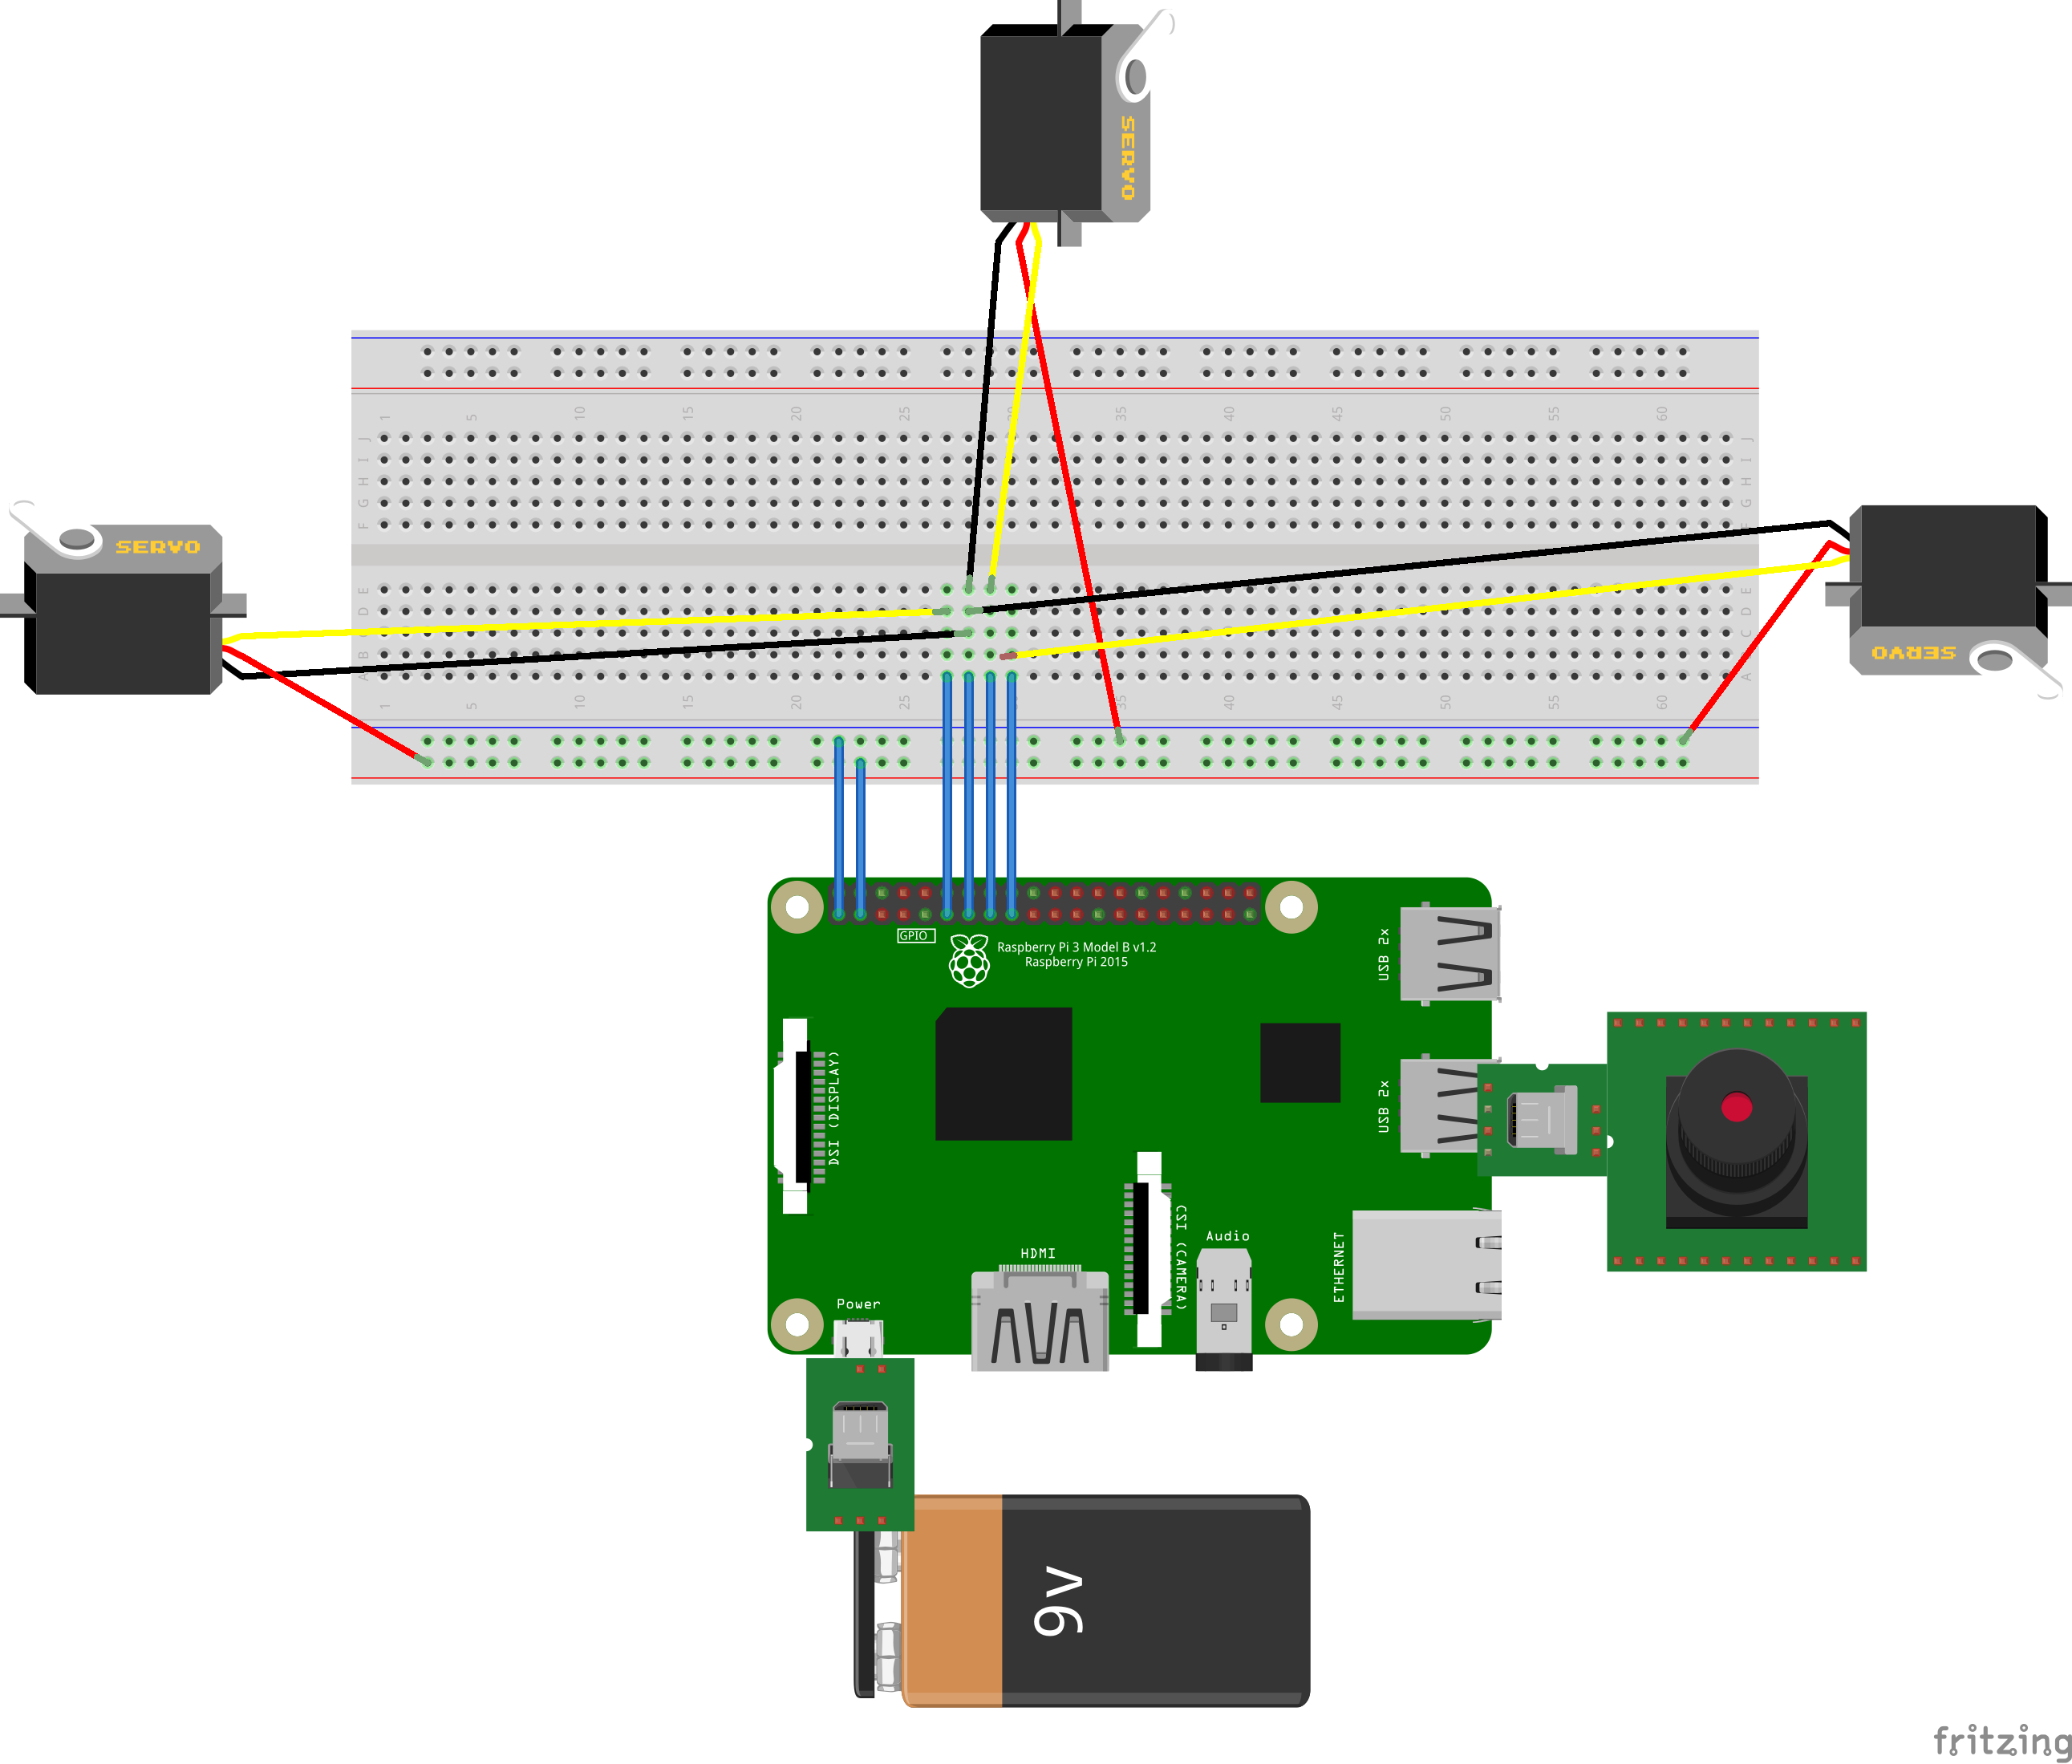
\includegraphics[width=.95\textwidth]{images/EsquemaServos.png}}
	}
	\caption{Esquema conexiones servos , cámara, Raspberry Pi 3}
\end{figure}\label{Figura conexiones robot}


\section{Router}
Para la comunicación entre el robot y el ordenador se necesita una red local,  para este trabajo la hemos creado haciendo uso de un router inalámbrico Xavi7968.
El router crea una red Wifi con el nombre de WifiRaspi3 y sin acceso a internet.

Cuando un dispositivo se conecta a una red, el router le asigna de forma automática una dirección IP que le identificará respecto a los otros dispositivos conectados a la misma red.\\
En este trabajo es necesario conocer la dirección IP de la Raspberry Pi 3 y del ordenador, y además necesitamos que siempre sea la misma, de esta forma será sencillo automatizar la conexión entre ambos.\\
Las direcciones IP las genera de forma automática un servidor DHPC(Dynamic Host Configuration Protocol), pero el router nos permite configurar dicho servidor y asignar a una dirección MAC una dirección IP. En términos más sencillos, podemos "reservar" una o varias direcciones IP de la red local y emparejar estas IPs a los dispositivos pertinentes.\\
Como podemos ver en la imagen \ref{Tabla DHPC} se ha configurado la tabla DHCP del router para asignar siempre la misma IP a la Raspberry y al equipo que utilizamos para conectarnos.

\begin{figure}[H]
	\centerline{
		\mbox{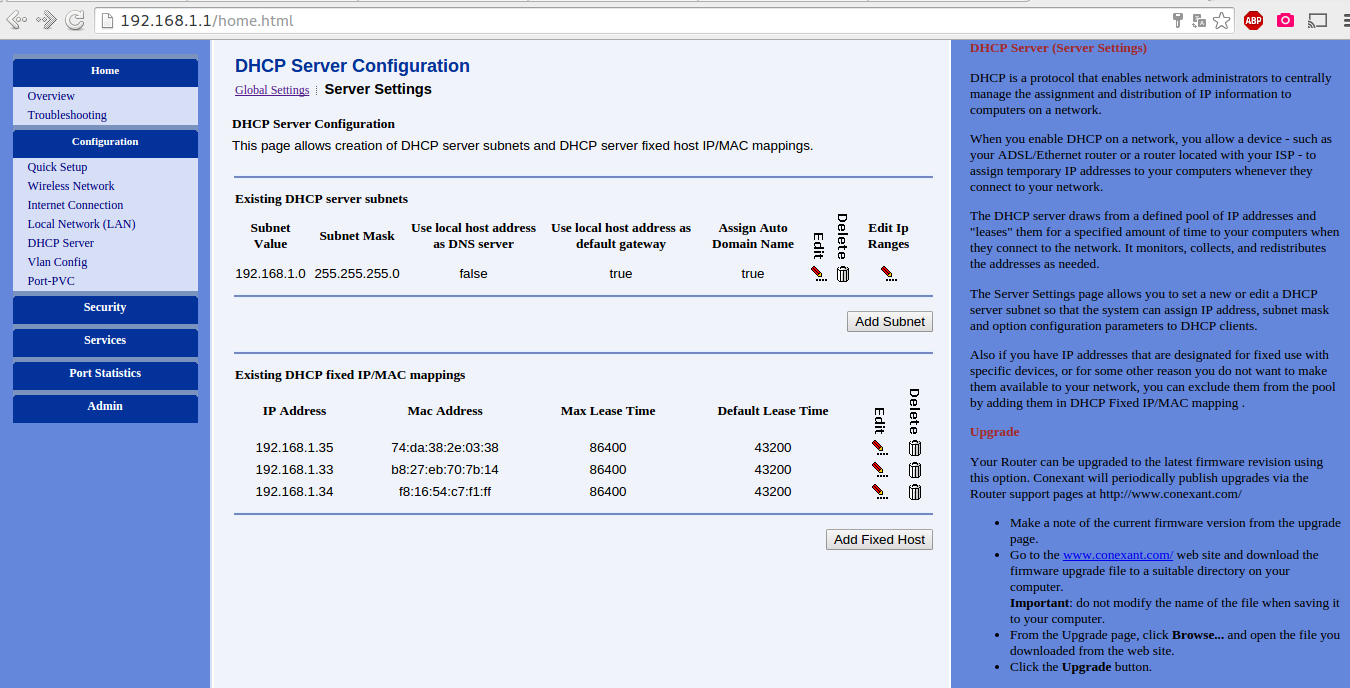
\includegraphics[width=.95\textwidth]{images/TablaDHCP2.png}}
	}
	\caption{Tabla DHCP del router con las parejas MAC-IP fijas}
\end{figure}\label{Tabla DHPC}

Una vez configurada la tabla DHPC, configuramos la Raspberry Pi 3 para conectarse automáticamente al router.\\
Esto se hace modificando el archivo \texttt{/etc/wpa\_supplicant/wpa\_supplicant.conf}, donde se ha añadido el nombre y la clave de la red creada por el router \ref{confwpa}. 

\begin{figure}[H]
	\centerline{
		\mbox{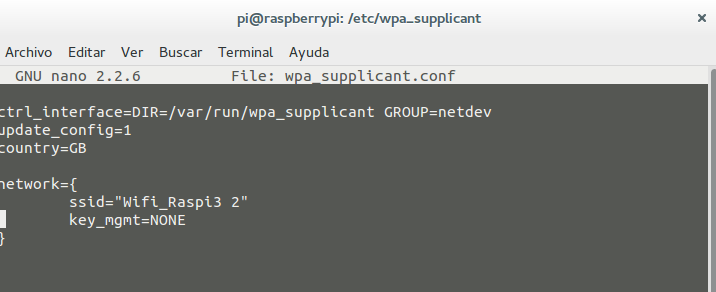
\includegraphics[width=.95\textwidth]{images/confRaspiWifi.png}}
	}
	\caption{Archivo de configuración de red Raspberry Pi 3}
\end{figure}\label{confwpa}
 
\newpage
\section{Oculus Rift}

Las Oculus Rift son unas gafas de realidad virtual creadas por Palmer Luckey.
Ha habido varias versiones de estas gafas.
La primera fue la DK1 (Develoment Kit 1), enfocada para programadores , que salió en abril de 2013. Esta versión se retiró del mercado poco antes de la presentación del segundo kit de desarrollo (DK2) en marzo de 2014.
Finalmente, en 2016 salió la versión para consumidor.\\
Para este proyecto se utiliza la versión \textbf{DK2}, ya que eran las gafas que teníamos disponibles.

Las gafas son un componente especialmente importante en este trabajo, ya que son el dispositivo que conecta al usuario con el entorno y el que transmite la información del robot al usuario y del usuario al robot.\\
Por ello las funciones clave de las Oculus Rift para el proyecto son:
\begin{itemize}
	\item Detección de la orientación: Las gafas llevan integradas sensores que permiten al ordenador conocer su orientación y transmitirla al robot.
	\item Sensación de inmersión (3D): dada la tecnología de las lentes de las Oculus Rift, es posible crear en el usuario una sensación de inmersión en el espacio en el que se encuentra el robot.
\end{itemize}

\subsection{Detección de la orientación}


Las Oculus Rift son capaces de detectar la \textbf{posición y orientación de la cabeza} del usuario.

Para la \textbf{posición} , las gafas llevan un conjunto de emisores infrarrojos en su superficie. La información enviada por dichos emisores es recogida por un sensor de infrarrojos que se asemeja a una cámara.\\
Para nuestro trabajo la posición no es relevante ya que, al estar orientado para personas con discapacidad motora,  se espera que el usuario se encuentre más o menos en la misma posición durante el uso del dispositivo.Por otra parte el usuario puede estar algo inclinado o incluso tumbado ya que, al no leer los sensores infrarrojos, el movimiento del robot no depende de la posición del usuario.


Por el contrario, conocer la \textbf{orientación} de la cabeza es esencial en este proyecto ya que el usuario enviará comandos al robot rotando la cabeza en el sentido que convenga en cada momento.\\Esta orientación se lee respecto a los ejes $X$, $Y$, y $Z$, como se puede ver en la figura \ref{Orientacion}  y se detecta gracias a los tres sensores que las Oculus Rift llevan integrados (giroscopio, acelerómetro y magnetómetro).

\begin{figure}[H]
	\centerline{
		\mbox{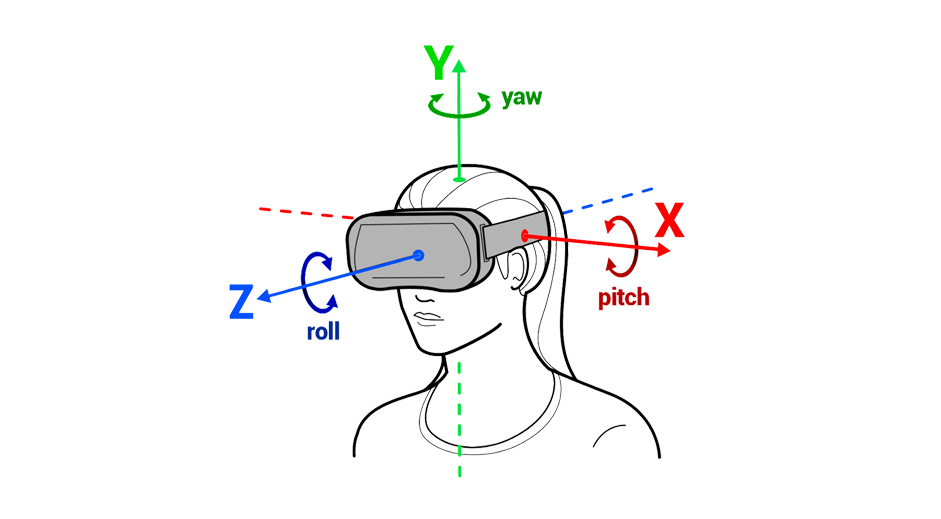
\includegraphics[width=3.55in]{images/headTrack.png}}
	}
	\caption{Ejes de giro}
\end{figure}\label{Orientacion}

Con el giroscopio y el acelerómetro se calcula la orientación respecto a los ejes $X$ y $Z$, mientras que el magnetómetro manda información del eje $Y$.\\Combinando la información de estos sensores a través de un proceso conocido como fusión de sensores se determina la orientación de la cabeza del usuario en el mundo real , y se sincroniza con la perspectiva virtual del usuario en tiempo real.\\
En este trabajo los giros de la cámara serán respecto a los ejes $X$ e $Y$ por lo que tampoco se recogerá información de la orientación de la cabeza respecto al eje $Z$
 
Se ha implementado un programa en phyton que recoge esa información y la traduce en comandos sencillos para mandarselos a la Raspberry. Para obtener esa información hacemos uso de la API de python (ovr \ref{subsec::OVR}) que se comunica con la librería de Oculus (LibOvr).










%Las Oculus Rift tienen integradas un giroscopio, un acelerómetro y un magnetómetro que manda constantemente información al ordenador, de forma que éste sabe en todo momento la orientación de las gafas.
%
%La técnoca para interpretar la señal de estos sensores se llama \textbf{fusión de sensores}
%
%A continuación se explica en qué consiste esta técnica.
%
%\paragraph{Fusión de Sensores }
%
%Como ya hemos mencionado, en las Oculus tenemos un giroscopio, un acelerómetro y un magnetómetro.
%
%Los dos primeros dan información acerca de la orientación respecto a los ejes X y Z, mientras que el magnetómetro mide la orientación respect al eje Y.
%
%Vamos a ver cómo funciona cada uno.
%
%El \textbf{giroscopio} de las Oculus mide el cambio de orientación de la cabeza a una velocidad de 1KHz.
%
%Una forma simplificada de calcular la orientación actual es:
%
%$$\text{Orientación actual } = \text{ Orientación anterior } + \text{ Diferencia horaria } \cdot \text{ Velocidad observada (giroscopio).}$$
%
%El problema está en que la cabeza puede rotar alrededor de tres ejes.
%
%\begin{figure}[h]
%	\centerline{
%		\mbox{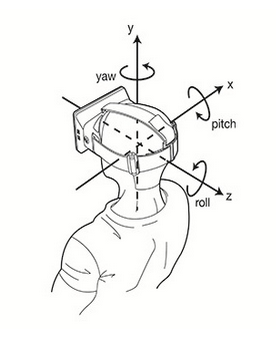
\includegraphics[width=3.00in]{images/headtracking.png}}
%	}
%	\caption{Ejes de giro}
%\end{figure}
%
%Vamos a suponer que solo rotase alrededor del eje Y y que el sensor captase una velocidad angular $w$ por segundo.
%
%Si tuviéramos 1000 sensores la fórmula de la orientación sería:
%
%$$\text{Orientación actual } = \text{ Orientación anterior } + 0,001 \cdot w$$
%
%Pero en el caso de las Oculus, al estar midiendo un objeto que se mueve en 3 ejes, el giroscopio da la velocidad angular respecto de los tres ejes, devolviendo un vector 3D ($w_1,w_2,w_3$)
%
%Al basar nuestro cálculo en el cálculo anterior, el error irá creciendo con el tiempo.
%
%Vamos a llamar \textit{tilt error} al error en la medición de los ángulos sobre los ejes XZ. El error sobre el eje Y se llamará \textit{yaw error}.
%
%El \textit{tilt error} se corresponde con nuestra sensación de lo que "está arriba", percepción que se basa en la gravedad.
%
%La gravedad se expresa con un vector de aceleración , por lo que utilizamos un \textbf{acelerómetro} para medirla.
%
%Nos encontramos con el inconveniente de que el acelerómetro no solo mide la gravedad. Para asegurarnos de que el momento en el que tomamos los datos de referencia solo estamos midiendo la gravedad, esperamos a que se den 2 condiciones:
%\begin{enumerate}
%	\item El acelerómetro nos devuelve una medida cercana a 9,8
%	\item El giroscopio nos devuelve una velocidad angular muy lenta (es decir, no estamos girando).
%\end{enumerate}
%
%En este momento sabemos que nos encontramos en una posición vertical y podemos corregir el error.
%
%\textbf{Cómo corregimos el error:}
%Supongamos que se dan las dos condiciones previas, y la posición que nuestro cálculo de orientación nos devuelve un vector $\vec{a}$, tal y como vemos en el dibujo.
%
%Tenemos el ángulo $\theta$ entre el eje Y y el vector $\vec{a}$ pero ¿cómo calculamos el eje de rotación para rotar $\vec{a}$ y corregir el error?
%
%Dicho vector debe ser perpendicular a $\vec{a}$ y al eje Y, y apoyarse en el plano XZ.
%
%Para encontrar el vector basta con hacer la proyección de $\vec{a}$ en el plano XZ, obteniendo así ($a_x, 0 , a_z$). Haciendo un vector perpendicular a éste obtenemos ($-a_z, 0 , a_x$). Y ya tenemos el eje de rotación que necesitábamos para corregir el error.
%
%\begin{figure}[h]
%	\centerline{
%		\mbox{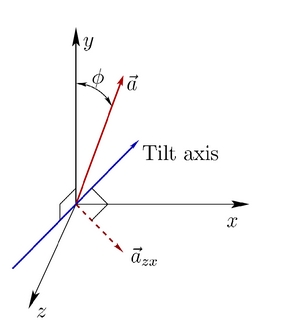
\includegraphics[width=3.00in]{images/ejestracking.png}}
%	}
%	\caption{Corrección del tilt error}
%\end{figure}
%
%
%\newpage
%\textbf{Error sobre el eje Y (yaw error)}
%
%Este error se basa en nuestra percepción de dónde está el norte.
%
%Para esto utilizamos el magnetómetro.
%
%El procesamiento de la señal del magnetómetro y la corrección del error es similar al tratamiento de la señal del giroscopio.

\subsection{Sensación de inmersión \_ 3D}

Una de las características más importantes de las Oculus Rift es su capacidad de reproducir un entorno virtual de tal forma que el usuario se sienta totalmente parte de él.

Esto lo hace usando un par de pantallas (una para cada ojo) que dividen la imagen en dos (Side by side - SBS). En cada pantalla hay un conjunto de lentes que modifican la imagen para crear el fenómeno de la estereopsis por el cual, a partir de dos imágenes ligeramente diferentes proyectadas en la retina de cada ojo, el cerebro es capaz de recomponer una tridimensional.

\subsection{OVR}\label{subsec::OVR}

Para desarrollar una aplicación integrada con las Oculus Rift utilizaremos la API OVR de python, que se encuentra en \url{https://github.com/cmbruns/pyovr}. Esta API está basada en otra API escrita en C que nos permite utilizar la librería LibOVR. Esta librería es la parte fundamental del SDK de Oculus.

Todo software que utilice OVR debe tener al menos 3 fases:
\begin{itemize}
	\item Inicialización.
	\item Bucle principal.
	\item Liberación de recursos y fin de proceso. 
\end{itemize}

\subsubsection{Inicialización}


Para inicializar la librería se utiliza la función \texttt{ovr.initialize(None)}. Esta función debe llamarse al principio de cualquier aplicación que utilice OVR.

Una vez inicializada la librería es necesario llamar a \texttt{ovr.create()}, que se comunica con el sistema operativo y crea el entorno necesario para gestionar las Oculus. Esta función devuelve dos valores: session(La sesión ovr) y luid( locally unique identifier). 

\subsubsection{Bucle principal}

En el caso de este trabajo, el bucle principal deberá leer la orientación de las gafas y enviarla al robot.

Para obtener la orientación es necesario recoger la información de los sensores de las Oculus Rift. Para ello OVR proporciona la función \texttt{ovr.getTrackingState()}, que devuelve una estructura \textit{TrackingState}. En esta estructura se encuentra el campo \textit{HeadPose}. Leyendo \textit{HeadPose.ThePose.Orientationx/y} se encuentra la orientación de la Oculus respecto a los ejes $x$ e $y$.

\subsubsection{Liberación de recursos y fin de proceso.}

Cuando finaliza la aplicación se deberá llamar a las funciones \texttt{ovr.destroy(session)} y \texttt{ovr.shutdown()}. Con estas funciones liberamos los recursos utilizados en la aplicación y apagamos la API.

\section{Diseño de conexiones entre módulos}

La arquitectura del proyecto es muy sencilla, como podemos observar en la siguiente imagen \ref{Fig::EsquemaConexiones}:

\begin{figure}[h]
	\centerline{
		\mbox{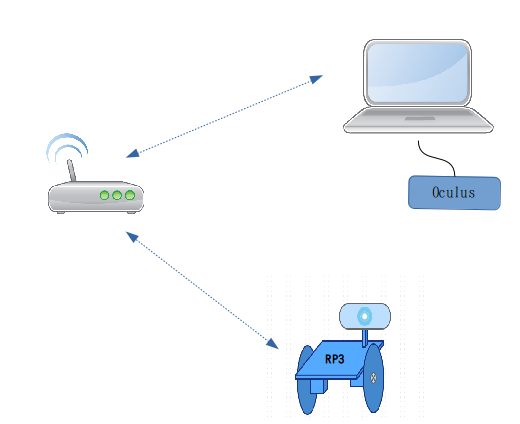
\includegraphics[width=.80\textwidth]{images/EsquemaConexiones.png}}
	}
	\caption{Esquema conexiones}
\end{figure}\label{Fig::EsquemaConexiones}


Todo el sistema, excepto las Oculus, se conecta a través de la red local creada por el router.\\
Para hablar de la conexión de las Oculus hay que especificar que nos referimos a la conexión de las gafas y la conexión de la cámara receptora de infrarrojos.\\
La cámara receptora de infrarrojos se conecta con el ordenador a través de un puerto USB y las gafas se conectan con la tarjeta gráfica a través de HDMI.

El resto de dispositivos, es decir, el ordenador y el robot, se encuentra dentro de la red local WifiRaspi3.De esta forma las el ordenador envía comandos de movimiento al router y el router al robot. Por otra parte la cámara (conectada por USB a las Raspberry Pi 3) transmite el video al robot y este lo manda en tiempo real al router, el router lo envía al ordenador de forma que el usuario podrá visualizarlo con las gafas de realidad virtual.


\newpage
\section{Esquema funcional}
A continuación se presenta un esquema funcional de todo el proyecto, en el que se puede ver cómo interacciona cada componente con los demás.

El esquema muestra un \textbf{ciclo retroalimentado}, ya que la información que manda el robot al usuario condiciona los comandos de movimiento que mandará el usuario al robot y viceversa.

\begin{figure}[h]
	\centerline{
		\mbox{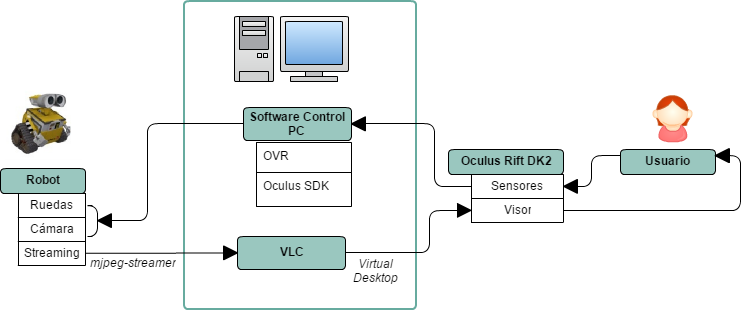
\includegraphics[width=1\textwidth]{images/EsquemaFuncional.png}}
	}
	\caption{Esquema funcional}
\end{figure}

Empezando el ciclo desde el \textbf{usuario}, vemos cómo el usuario le manda información a los sensores, esto es, cuando el usario mueve la cabeza, los sensores de las \textbf{Oculus} perciben el cambio de orientación y le mandan los datos al PC.

El PC recoge los datos a través del SDK de Oculus. Estos datos son interpretados en un \textbf{software de control} utilizando la API OVR. Una vez interpretados los datos se envían los comandos convenientes a los motores del \textbf{robot}. Estos comandos llegarán a los motores de las ruedas o al motor de la cámara, dependiendo de la nueva orientación de la cabeza del usuario.

A la vez que ocurre este proceso el robot está enviando un video del entorno en tiempo real al PC. Esta transmisión se hace a través de la librería mjpeg-streamer y es recogida en el PC por el reproductor de video \textbf{VLC}.

Para que el video llegue al visor de las Oculus Rift se utiliza Virtual Desktop, como ya se dijo en la sección anterior. De esta forma el usuario podrá visualizar lo que ve el robot a través de la Oculus y mover el robot hacia donde desee.



\newpage
\chapter{Desarrollo e implementación}

Una vez definidos los objetivos y requisitos que debe cumplir el trabajo y haber diseñado el sistema y las conexiones se ha desarrollado el sistema basado en todo lo anterior.\\
En esta sección se explicará cómo hemos desarrollado e integrado las distintas funcionalidades para conseguir el proyecto final.Ya que el proyecto es tan amplio e integra tantas tecnologías,para clarificar la explicación se ha dividio el desarrollo en tres bloques:
\begin{itemize}
	\item Construcción del Robot
	\item Streaming 
	\item Control del Robot
\end{itemize}
Cada bloque se desarrollará a lo largo del capítulo pero, para tener una idea global,primero se van a resumir brevemente.

La \textbf{construcción del robot} se ha hecho acorde con el diseño y los requisitos del mismo, es decir, con dos ruedas que le permitan transportarse, un soporte para la Raspberry Pi 3 y un soporte para la cámara.\\
Este diseño se basa en un diseño de otro trabajo fin de grado de un alumno de la UAM, añadiendo para este proyecto los accesorios necesarios.

Para conseguir \textbf{transmitir a las Oculus el video en tiempo real} es necesario que la Raspberry recoja el video de la cámara y lo transmita al ordenador.A su vez el ordenador recojerá el video, lo transformará a formato SBS y lo reproducirá en las Oculus Rift. 

El último bloque es el \textbf{control del robot}. El primer paso para poder enviar comandos de control es leer la señal de los sensores de las Oculus Rift (giroscopio, acelerómetro y magnetómetro) para saber la orientación de la cabeza del usuario.\\
Una vez que obtenemos dicha información se procesa y transforma en datos útiles para el robot se transmite a las Raspberry Pi con la mínima latencia posible.\\
Cuando el robot recibe los datos los convierte en instrucciones para mover los servomotores, es decir, en pulsos que le indican un cambio de posición.
	

\section{Construcción del Robot}
Como se ha dicho en la sección de diseño, el robot está construido basándose en el diseño de un robot de un trabajo anterior.\\
Para este proyecto se han añadido dos componentes adicionales:

\begin{itemize}
	\item \textbf{Soporte de la cámara:} este soporte debe servir como pinza de agarre de la cámara y a su vez debe estar unida al servomotor que mueve la cámara.
	\item \textbf{Batería portátil:} Ya que el robot debe ser inalámbrico, de acuerdo con los requisitos del proyecto, en su estructura hay cabida para una batería portatil que alimenta la Raspberry Pi 3 y a través de ésta, la cámara y los tres servomotores.
\end{itemize}

\subsection{Soporte de la cámara}
El soporte de la cámara se ha construido en base a que la cámara debía encontrarse a una altura algo elevada sobre la base del robot para poder rotar sin encontrarse con obstáculos y para lograr un mayor ángulo de visión. Otro requisito que tiene que cumplir el soporte es el de dar lugar a que se coloque el servomotor que controla el movimiento de la cámara.\\
En base a estas dos condiciones se ha ideado un soporte con dos piezas: Un soporte vertical y una pinza de agarre. 

\begin{itemize}
	\item Soporte vertical $\rightarrow$ En esta pieza se coloca el servomotor que controla el movimiento de la cámara.
	
	\item Pinza de agarre $\rightarrow$ Se utiliza para unir la cámara con el servomotor que a mueve.
\end{itemize}

Ambas piezas han sido impresas en plástico con la impresora 3D del Club de Robótica de la Universidad Autónoma de Madrid.\\
Para realizar el diseño 3D de la pinza de agarre se ha utilizado el programa de diseño 3D Blender.\\
En este programa se diseña gráficamente la pieza y genera una archivo \texttt{.stl}, tal y como se muestra en la imagen \ref{fig::blender}. 
\begin{figure}[H]
	\centerline{
		\mbox{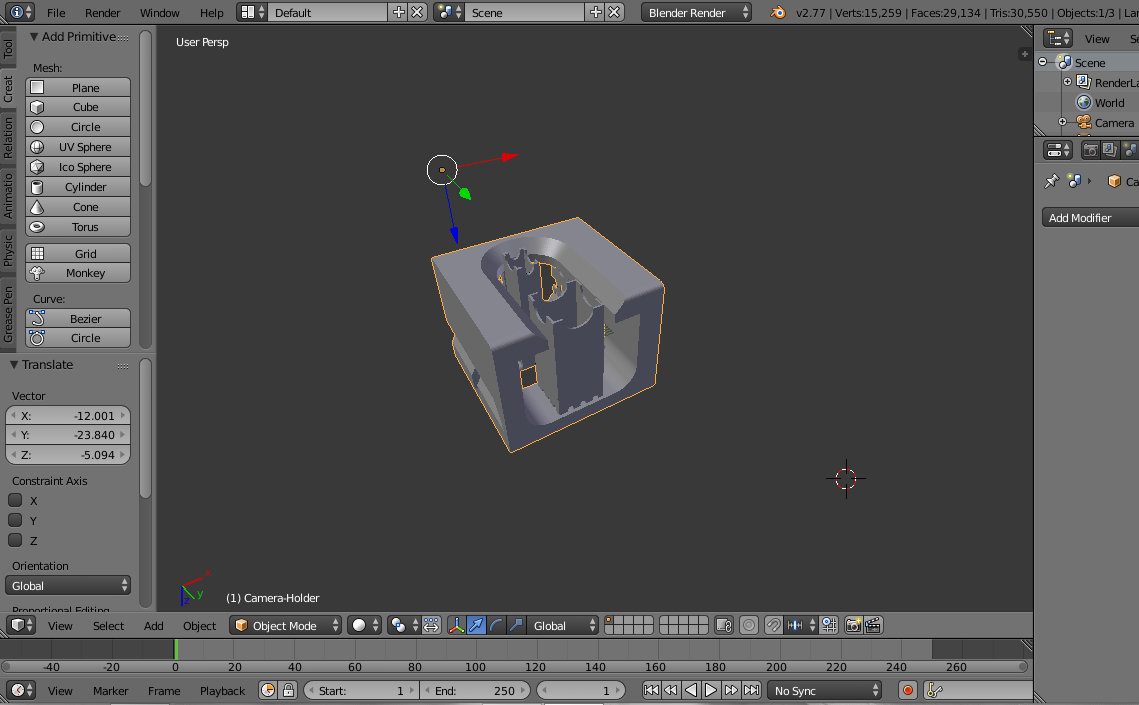
\includegraphics[width=.80\textwidth]{images/cameraBlender.png}}
	}
	\caption{ Diseño 3D de la pinza de agarre en Blender}
\end{figure}\label{fig::blender}

Una vez creado el fichero \texttt{.stl} utiliza un Cura, un programa que nos permite seleccionar los parámetros de configuración deseados para la impresión de la pieza, como por ejemplo la densidad o el tamaño. Una vez elegida la configuración, Cura genera el archivo \texttt{.gcode}. Este tipo de archivos son los que lee la impresora 3D y consiste en una serie de instrucciones de movimiento para los servomotores que controlar el estrusor y el ventilador de la impresora.\\
En la imagen \ref{Cura} podemos ver la interfaz de Cura, la base azul del centro representa la base de impresión de la impresora. A la izquierda se pueden ver algunos de los parámetros de configuración.

\begin{figure}[H]
	\centerline{
		\mbox{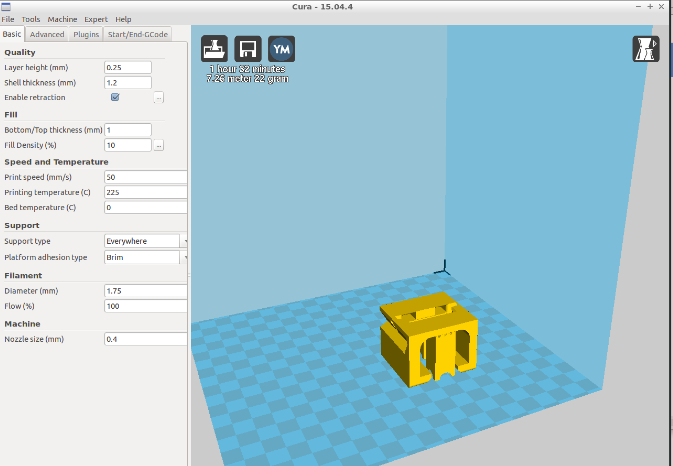
\includegraphics[width=.75\textwidth]{images/Cura2.png}}
	}
	\caption{Imagen de la configuración del Cura para enviar la Pieza de agarre a la impresora 3D}
\end{figure}\label{Cura}
 
\section{Streaming}
El segundo bloque es el streaming, es decir, la transmisión del video que captura la cámara al ordenador y su posterior reproducción en las Oculus Rift.\\
La Raspberry Pi3 se encargará de recoger el video de la cámara y transformarlo en paquetes de datos IP para poder transmitirlos a una dirección de la red local.\\El ordenador va recogiendo el streaming de la dirección donde lo envía la Raspberry Pi 3 y lo reproduce en las Oculus.

\subsection{Raspberry Pi3}
La Raspberry Pi, tiene conectada por usb la cámara que se utiliza para capturar el video.\\
Para recoger el video y mandarlo en tiempo real utilizamos la aplicación de software libre mjpeg-streamer, disponible en github. \url{https://github.com/jacksonliam/mjpg-streamer}

\textbf{Mjpeg-streamer} es una aplicación en linea de comandos que permite crear un servidor, para obtener frames JPG desde una cámara compatible con la aplicación y transmitirlos como M-JPEG mediante protocolo HTTP. Está diseñada para dispositivos con recursos limitados, en téminos de CPU y RAM.\\
Soporta la compresión por hardware (GPU) de la cámara, en nuestro caso H.264 Advanced Video Coding (AVC) Standard, que es la compresión utilizada por la Webcam Logitech, lo cual permite reducir drásticamente el uso de la CPU de este servidor, haciendo está aplicación un servicio ligero.\\
Esta característica hace de esta aplicación una buena candidata para el objetivo que perseguimos en este trabajo, ya que la compresión y transmisión del streaming se hace a tiempo real.

En la imagen \ref{fig::mjeg} se muestra el uso de recursos de la aplicación mjpeg-streamer.


\begin{figure}[h!]
	\centerline{
		\mbox{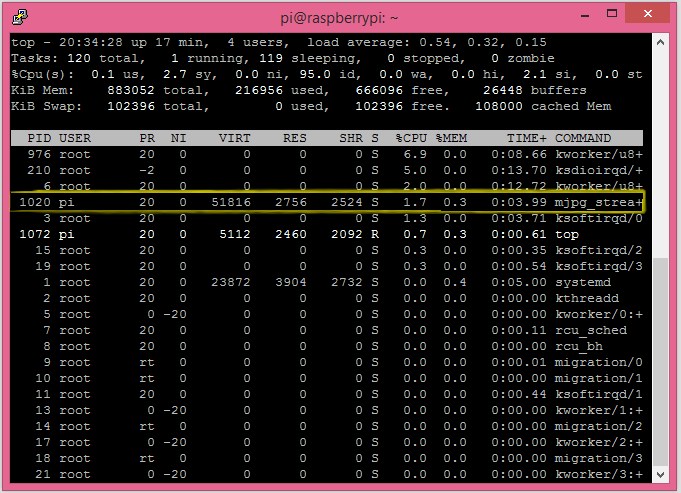
\includegraphics[width=.80\textwidth]{images/UsoCPUMjpeg.png}}
	}
	\caption{Uso de CPU del programa Mjpeg-Streamer por el que se hae el streaming de video}
\end{figure}\label{mjpeg}

La aplicación arranca en la Raspberry Pi cuando ejecutamos el siguente comando: \texttt{./mjpg\_streamer -i "./input\_uvc.so -d /dev/video0" -o "./output\_http.so -w ./www"}.\\Para entender este comando hay que explicar primero el funcionamiento de mjpeg-streamer. La aplicación se basa en unos plugins de entrada y salida. Es decir, un plugin (de entrada) copia las imágenes JPEG a un directorio de acceso global, mientras que otro plugin (de salida) procesa las imágenes y las emite de acuerdo a los estándares MPG existentes.\\ En el comando que arranca la aplicación estamos especificando:
\begin{itemize}
	\item \textbf{ -i "./input\_uvc.so}: Este es el plugin de entrada, que captura los frames JPG de la cámara conectada.
	\item \textbf{-o "./output\_http.so -w ./www"}: El plugin de salida (\texttt{./output\_http.so}), es un servidor web HTTP 1.0, que emite el video en los estándares M-JPEG. El directorio de la aplicación web de mjpeg-streamer se especifica con la opción \texttt{-w ./www}
	\item \textbf{mjpg\_streamer}: instrucción que transmite los frames desde el plugin de entrada al de salida.
	\item \textbf{-d /dev/video0}: especifica la cámara que se va a utilizar ya que la Raspberry Pi 3 tiene dos puertos usb.
\end{itemize}

En el momento en que se ejecuta el comando la Raspberry empezará a coger el video de la cámara y transmitirlo en tiempo real a la siguiente url: \texttt{http://192.168.1.33:8080/stream.html} y muestra información sobre el streaming por terminal.\\
En la imagen \ref{fig::outmjpeg} vemos un ejemplo de dicha información y en la imagen \ref{fig::stream} vemos la dirección de la red local donde la Raspberry Pi está transmitiendo el video.

\begin{figure}[H]
	\centerline{
		\mbox{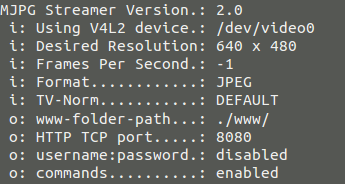
\includegraphics[width=.80\textwidth]{images/Streamingcomando.png}}
	}
	\caption{Ejecución del comando para iniciar el streaming}
\end{figure}\label{fig::outmjpeg}


\begin{figure}[H]
	\centerline{
		\mbox{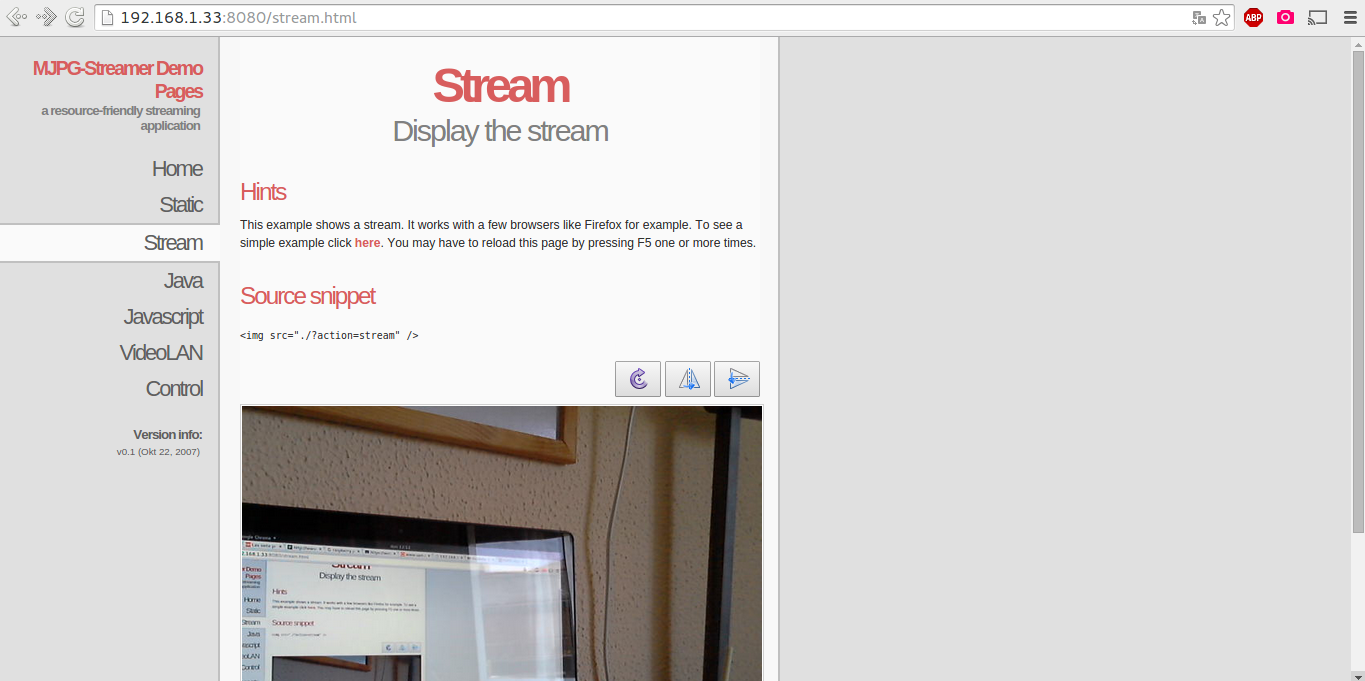
\includegraphics[width=.80\textwidth]{images/pagStream.png}}
	}
	\caption{Página html donde se recibe el streaming a tiempo real desde la Raspberry }
\end{figure}\label{fig::stream}


\subsection{Ordenador}
Una vez el robot es capaz de transmitir video a tiempo real a una dirección de la red local, solo falta desarrollar las funciones del ordenador.\\
El PC debe capturar el video de la red local y reproducirlo en las Oculus Rift.\\
El ordenador , conectado a la red local a través del router,accede a la IP donde mjpeg-streamer está retransmitiendo el video y lo recoge a través del reproductor de video  \href{http://www.videolan.org/vlc/}{\textcolor{blue}{VLC}}.

\textbf{VLC media player} es un reproductor multimedia libre y de código abierto. Tiene dos características que lo hacen idóneo para este proyecto: Es capaz de capturar y reproducir video de una dirección de red y puede dividir la imagen del video en dos pantallas.

Por lo tanto se configura VLC para que el medio de reproducción sea la ubicación de red donde se está transmitiendo el video del robot \texttt{http://192.168.1.33:8080/?action=stream}.\\
Posteriormente dividimos el video en dos pantallas exactamente iguales para poder verlo desde las Oculus en modo SBS (Side by Side).\\Ambas configuraciones y el resultado pueden verse en la figura \ref{figstream}

\begin{figure}[H]
	\centering
	\subfigure[Medio de reproducción-Ubicación de red]{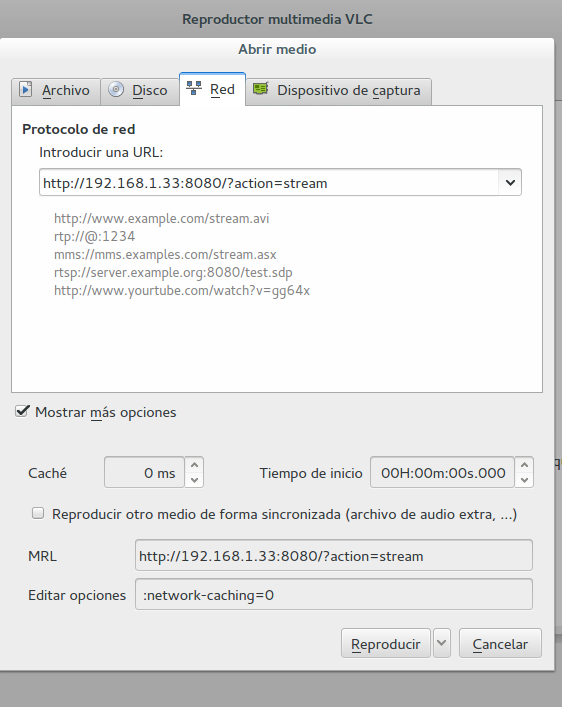
\includegraphics[width=60mm]{images/confVLC.png}}
	\subfigure[División de imágenes]{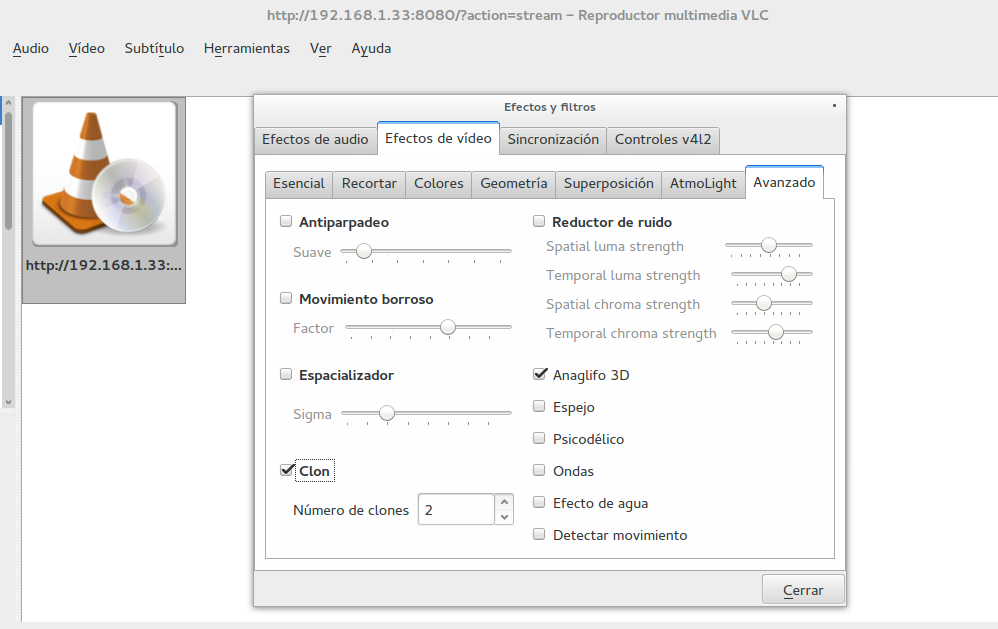
\includegraphics[width=60mm]{images/confSBS.png}}\\
	\subfigure[Reproducción SBS]{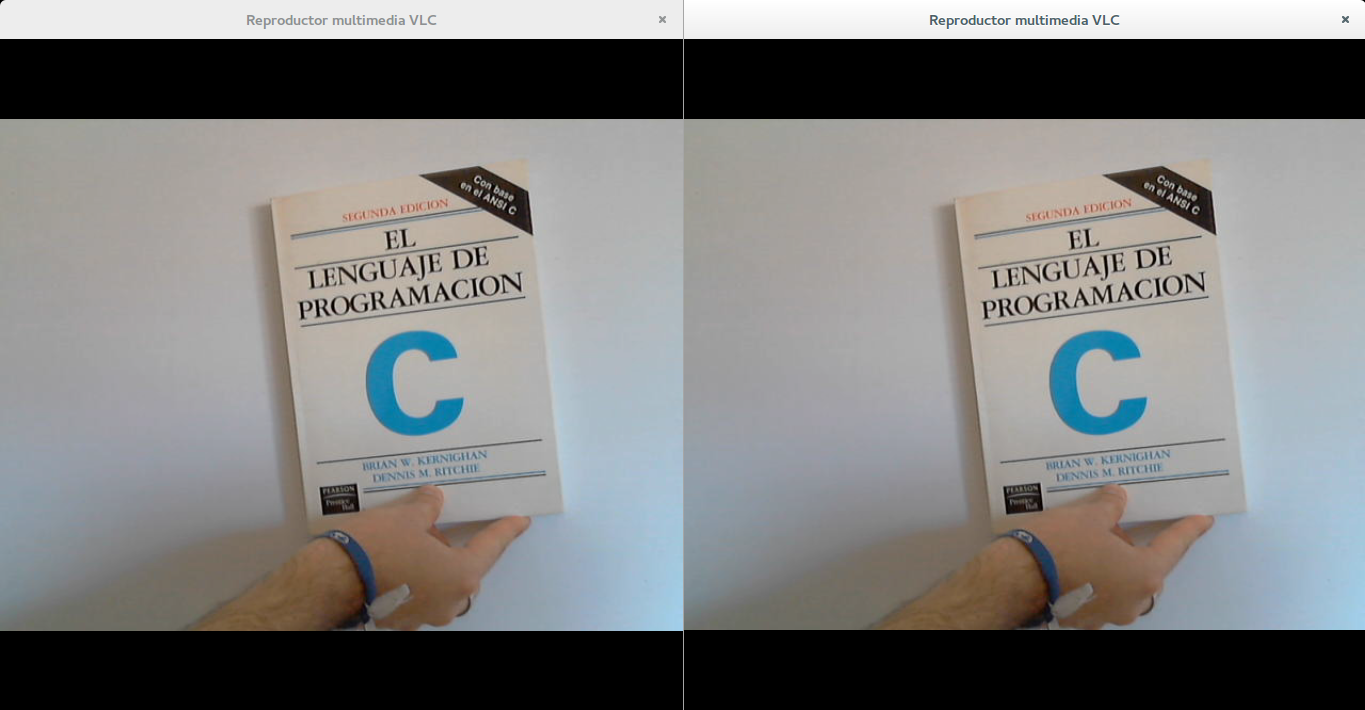
\includegraphics[width=120mm]{images/sbsVLC2.png}}
		\caption{Configuración y resultado de la reproducción de video en VLC} \label{figstream}
\end{figure}

Una vez capturado el video en el ordenador solo queda visualizarlo en las Oculus Rift.\\
Para ello hemos instalado en el PC el \href{http://store.steampowered.com/app/382110/}{\textcolor{blue}{Virtual Desktop}}. 

\textbf{Virtual Desktop} es una aplicación desarrollada por Oculus Rift y  HTC Vive para utilizar las Oculus Rift en Windows.\\
Permite ver el escritorio desde las Oculus, pudiendo configurar efectos como ver las imagénes SBS o cambiar el entorno en el que te encuentras (el espacio, una sala de cine...)\\También te permite ver videos descargados en el ordenador y reproducir videos 360.\\
La funcionalidad que es interesante para este trabajo es la de ver la pantalla del ordenador desde las Oculus con SBS, para visualizar el video que se está reproduciendo en VLC a tiempo real.\\
De esta forma, si ponemos en video en pantalla completa en el PC y configuramos Virtual Desktop correctamente, el video se reproducirá en la Oculus Rift a tiempo real.


%\begin{figure}[h]
%	\centerline{
%		\mbox{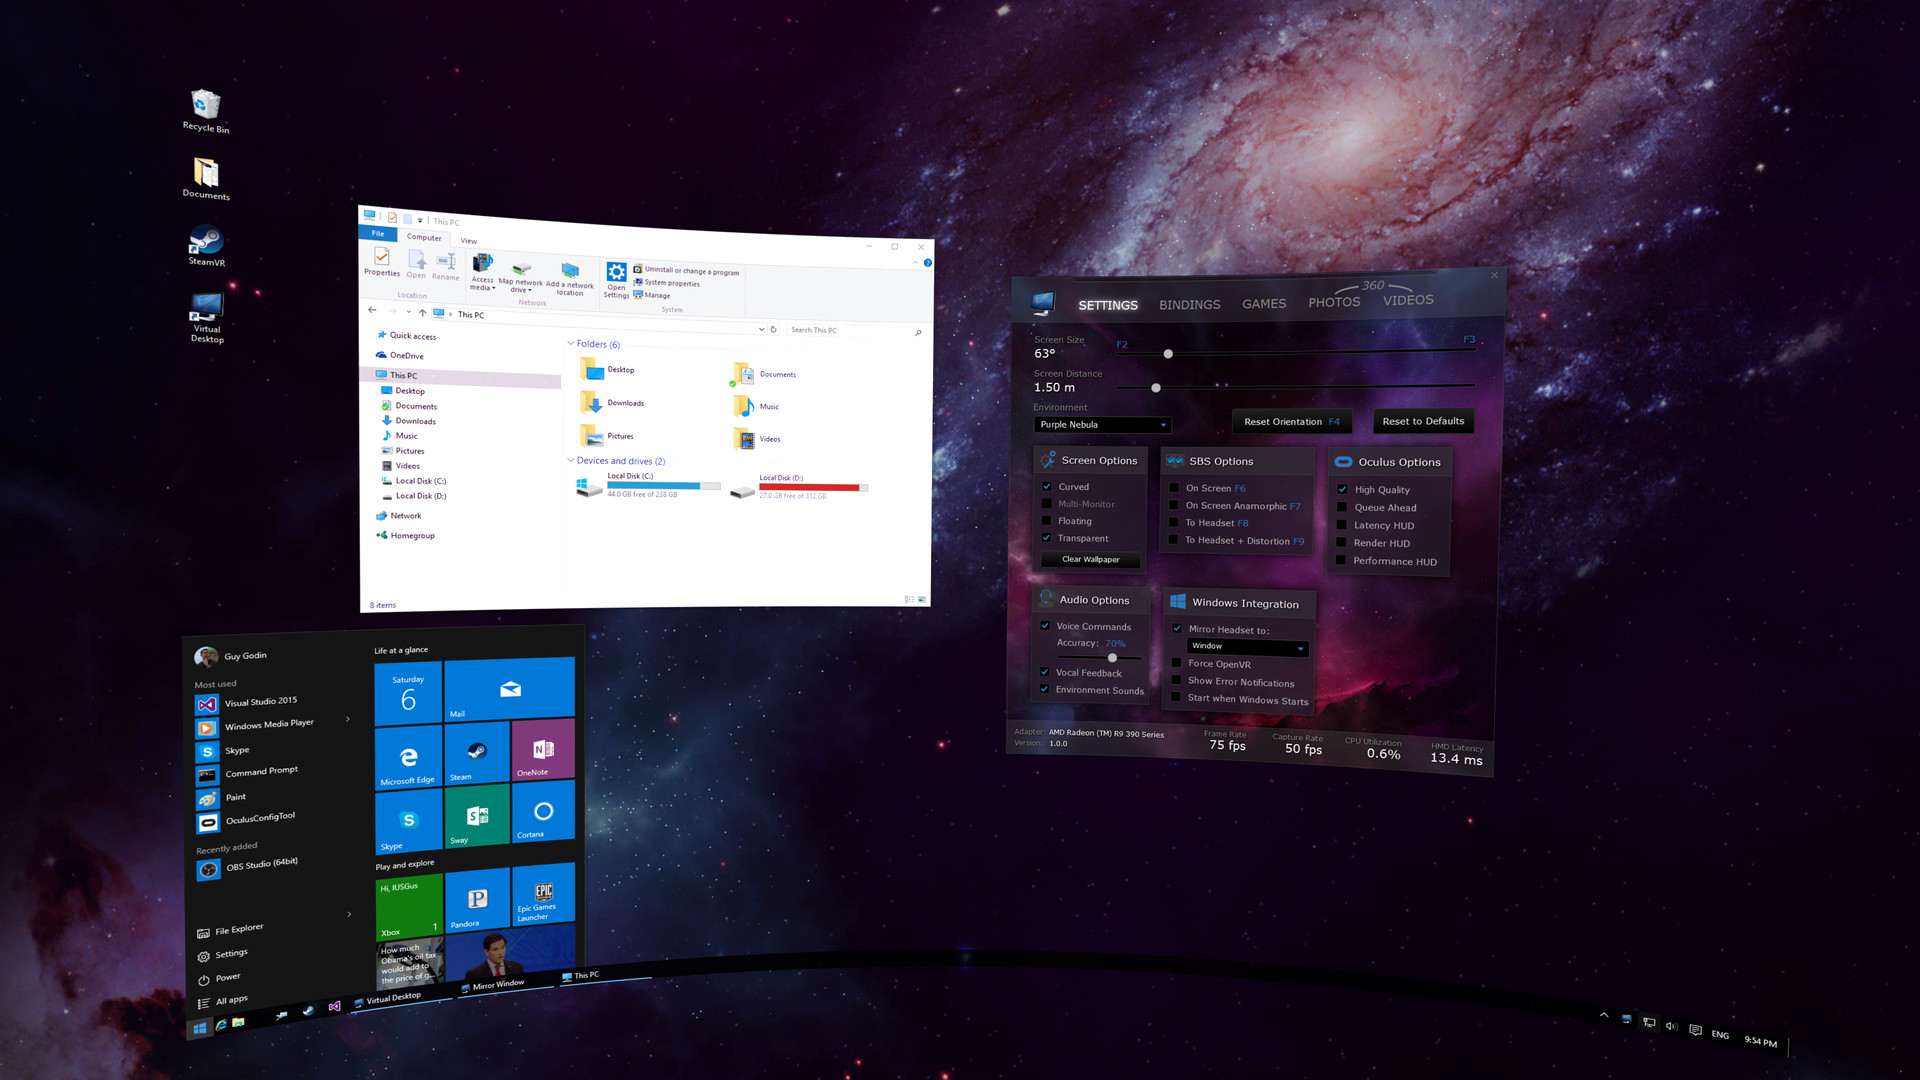
\includegraphics[width=3.00in]{images/VirtualDesktop.jpg}}
%	}
%	\caption{Virtual Desktop}
%\end{figure}



\section{Control del Robot}
El último bloque de desarrollo que queda por implementar es el control del robot. Por control del robot se entiende el control del movimiento de los tres servos que lo componen. Dos para las ruedas laterales que permiten que el robot se transporte y uno para la cámara, que permite que esta rote respecto al eje horizontal.\\
Estos movimientos se basarán en el movimiento de las Oculus, que llevará puestas el usuario.\\
Por lo tanto el control del robot se divide en tres acciones:
\begin{itemize}
	\item Recogida y procesamiento de la información que mandan las Oculus al ordenador $\rightarrow$ Esto se hará mediante la utilización de la API de Python \texttt{OVR}.
	
	\item Envío de la información procesada a la Raspberry Pi 3 $\rightarrow$ Para ello el ordenador abrirá dos sockets a través de los cuales mandará los datos al robot
	
	\item Movimiento de los servomotores
\end{itemize}
\subsection{Recogida y procesamiento de la información que mandan las Oculus al ordenador}

Para recoger desde el ordenador la información que mandan las Oculus utilizamos la API de Oculus (\texttt{OVR}), explicada en el capítulo de Diseño \ref{subsec::OVR}.\\
Con las funciones proporcionadas por OVR se puede conocer la orientación de la cabeza del usuario respecto a los ejes $x$ e $y$.\\
La información obtenida sobre la orientación respecto al eje $y$ servirá para mover los servos que hay en las ruedas del robot, mientras que la información de $x$ servirá para mover la cámara.\\
Los datos referentes a la posición de las Oculus se convierten grados, lo que facilita el control posterior de la posición de los servomotores.\\
El ordenador crea un servidor y abre dos sockets distintos, uno para la información de $x$ y otro para la de $y$.


De esta forma manejamos los dos movimientos de forma independiente.


\begin{figure}[h!]
	\centerline{
		\mbox{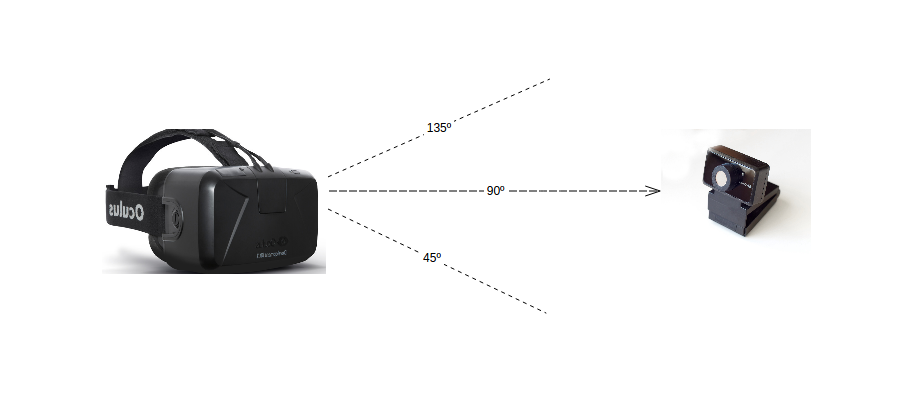
\includegraphics[width=.80\textwidth]{images/Oculusgrados2.png}}
	}
	\caption{Posición de las Oculus respecto al eje X}
\end{figure}
\newpage
\paragraph{Envío de la información procesada a la Raspberry Pi 3}


Para el control del movimiento del robot es necesario que el ordenador le mande los datos referentes a la posición de las Oculus de forma automática, inmediatamente después de procesarlos.

Con este fin, desde el mismo programa donde se recibe y procesan los datos de las Oculus, el ordenador abre dos sockets, y se queda a la espera de que el robot se conecte.

Recordemos que el ordenador y la Raspberry Pi 3 están dentro de la misma red local (WifiRaspi3), y que ambos tenían IP fija.

La apertura de sockets por parte del ordenador se hace de la siguiente forma:

\lstset{language=python, breaklines=true, basicstyle=\footnotesize}
\begin{lstlisting}[frame=single]

	host = "192.168.1.35"    #IP asignada al ordenador
	port = 4446       #movimiento de la camara
	port2 = 4447      #movimiento de las ruedas

	s = socket(AF_INET, SOCK_STREAM)
	s2 = socket(AF_INET, SOCK_STREAM)

	s.bind((host,port))
	s2.bind((host,port2))

	s.listen(5)
	s2.listen(5)

	q,addr = s.accept()
	q2,addr2 = s2.accept()

\end{lstlisting}

De esta forma, cada vez que se recibe y procesan datos referentes a la posición de las Oculus, se dividen en información para la cáma e información para las ruedas y se ejecutna las instrucciones \texttt{ q2.send(data)}  y \texttt{ q.send(data)} para mandar los datos.
\subparagraph{Recepción de los datos en el robot}

La Raspberry tiene dos programas (uno para las ruedas y otro para la
cámara) que están escuchando continuamente lo que manda el ordenador y en
cuanto recibe el comando lo manda a los servos.

Para ello, al iniciarse cada programa, se conectan al socket correspondiente
\lstset{language=python, breaklines=true, basicstyle=\footnotesize}
\begin{lstlisting}[frame=single]
	host = "192.168.1.35"
	port=4447
	s=socket(AF_INET, SOCK_STREAM)
	s.connect((host,port))
\end{lstlisting}

Y se ponen a escuchar hasta que les llegan los datos.

Una vez que tiene los datos los transforma en comandos válidos para los servomotores,tal y como se explica en el siguiente apartado, les manda la instrucción y vuelve a escuchar.


\subsection{Movimiento de los servomotores}


Como ya se indicó en la sección (seccion de los servos,PWM, etc..) el movimiento de los servos se controla con una señal PWM (Pulse Width Modulation).

Por ello utilizamos la librería RPi.GPIO, que ofrece funciones para PWM.

Hay dos parámetros principales para determinar el pulso que se envía al motor:
\begin{itemize}
	\item \textbf{Frecuencia} : veces por segundo que se genera el pulso.
	\item \textbf{Duty cycle} : indica el porcentaje de tiempo que dura la señal cuadrar en relación con el periodo.
	$$DutyCycle = \frac{PW}{T}\cdot 100$$
	Donde $PW$ indica el ancho de pulso (pulse width) y $T$ es el periodo.
	
\end{itemize}

Para controlar los servomotores del robot se fija una frecuencia de 50 Hz, es decir, $T = \frac{1}{50} = 20 ms$.
En las especificaciones de los servos se indica que el rango de $PW$ es $0.5 \text{ ms } \sim 2.5\text{ ms }$ y con esto ya podemos calcular el Duty Cycle adecuado para cada acción.

En la siguiente imagen se muestra cómo varía la posición de los motores según el pulso que se le envíe.

\begin{figure}[h!]
	\centerline{
		\mbox{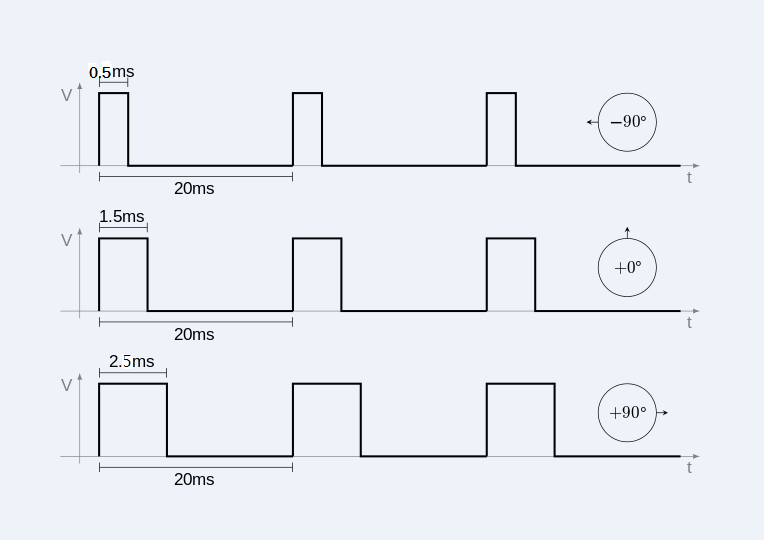
\includegraphics[width=.80\textwidth]{images/PWMServos.png}}
	}
	\caption{Relación entre el PW y la posición de los servomotores}
	\label{figPWM}
\end{figure}
%Por lo tanto, si mandamos un pulso cercano a $0.5$ ms, el servo girará a gran velocidad hacia la izquierda, mientras que si el pulso es cercano a $2.5$ ms girará hacia la derecha. A medida que el pulso se va acercando a $1.5$, el motor perderá velocidad. 

Recordemos que estos valores son orientativos, pudiendo variar ligeramente según el servomotor.

%Veamos un ejemplo para clarificar esto:
%
%\subparagraph{PWM- Frecuencia:50Hz , DutyCycle $50\%$}
%
%
%
%Si fijamos una frecuencia de 50Hz estaremos mandando una señal de 50 pulsos por segundo, es decir, un pulso cada $0.02$ segundos.
%
%Al poner un DutyCycle al $50\%$ estamos estableciendo que durante esos $0.02$ segundos el pulso estará $0.01$ segundos en posición "High" y el resto del tiempo en posición "Low".
%
%
%\subparagraph {PWM- Frecuencia:50Hz , DutyCycle $80\%$}
%
%Si fijamos una frecuencia de 50Hz, como la del ejercicio anterior pero por el contrario ponemos un DutyCycle del $80\%$ tendremos:
%\begin{itemize}
%	\item 1 pulso cada $0.02$ segundos
%	\item El pulso estará en posición "high" el $80\%$ del tiempo ($0.016$ segundos) y en posición "low" los otros $0.004$ segundos restantes.
%\end{itemize}



La Raspberry Pi recibe a través de los sockets información sobre la orientación de la cabeza sobre el eje y o x.


Esta información se procesa de forma distinta según si queremos mover el servo de la cámara o las ruedas del robot.

Esto es porque los servos de las ruedas son de rotación continua, a diferencia que el de la cámara.

\subsubsection{\textbf{Control de los motores de las ruedas del robot}}

Los motores que mueven las ruedas del robot son dos servomotores de rotación continua. El funcionamiento de los servomotores de rotación continua ya se ha explicado en la sección de análisis.

Recordamos muy brevemente que en los servomotores de rotación continua, la pulsación que le mandas al motor no indica la posición en la que debe colocarse si no la dirección y velocidad a la que debe rotar.

Por lo tanto si se envía un pulso cercano a $1.5$ ms, el motor girará muy despacio. Por el contrario, si el pulso es cercano a $0.5$ o $2.5$ ms, el motor se moverá a mayor velocidad.

Para controlar nuestro robot se ha fijado una velocidad constante de giro en base a pruebas experimentales que se explicarán en la sección de Pruebas y resultados.

De esta forma para rotar nuestro robot hasta una posición concreta la variable no es la velocidad si no el tiempo durante el que rotan los motores.

Para girar el robot hacia la derecha el usuario enviará la señal de "rotar hacia la derecha" y el robot empezará a rotar en esa dirección hasta recibir la señal de "parar".

%Para calcular dicho tiempo se midió experimentalmente cuanto tardaba el robot en girar 90º. El resultado fueron 0.5 segundos por lo que 
%$$90 / 0.5 = 0,005555556 \text{ segundos en girar un grado}$$
%
%De esta forma, cuando el robot recibe una posición en grados desde el ordenador ejecuta las siguientes instrucciones:
%
%
%$\begin{cases}
%\text{Grados recibidos del ordenador = g}\\
%dif = |posActual-g|\rightarrow\text{ Se calcula el número de grados que tiene que moverse}\\
%\text{Rotar motores derecho e izquerdo}\\
%time.sleep((dif*0.005555) \rightarrow \text{ Rotamos el tiempo necesario alcanzar la posición}\\
%\text{Parar motores derecho e izquerdo}
%\end{cases}$



\subsubsection{\textbf{Control del motor de la cámara del robot}}

La cámara se mueve gracias a un servomotor cuyo rango de movimiento va de -90 a 90 grados.

Este motor se mueve por pulsos, tal y como se explica en la sección de Análisis.

La Raspberry recibe un ángulo que indica hacia donde están orientadas las Oculus en ese momento.

Para transformar este ángulo el pulso(PWM) correspondiente debemos tener en cuenta el rango de pulsos del motor que se está utilizando.

Como vemos en la figura \ref{figPWM}, un pulso de $1.5$ ms equivale a la posición del motor que señala el ángulo 0, de la misma manera para que el motor esté orientado hacia el ángulo -90 deberemos mandar un pulso de $0.5$ ms y para orientarlo en el ángulo de 90mandaríamos un pulso de $2.5$. Por lo tanto , un pulso de diferencia implica 90 grados de diferencia.

Con estos datos es sencillo encontrar una fórmula de conversión de grados a pulsos:

$$p = \frac{g}{90} + 1'5$$
Siendo $p$ el pulso que debo mandar al servomotor para que rote hasta la posición señalada por el grado $g$.

Asi podemos convertir los ángulos en pulsos PWM y mover la cámara hacia la dirección deseada.

\paragraph{Control del Robot por parte del usuario}

El las anteriores secciones se ha explicado el funcionamiento interno del control de movimientos del robot.

En este nuevo apartado se presenta cómo debe utilizar el usuario este producto, qué rango de movimiento tiene y cómo puede hacer avanzar el robot.

\subsubsection{\textbf{Instrucciones de mando}}

Como se especifica al inicio de este trabajo, el robot estará controlado exclusivamente por el movimiento de cabeza del usuario.

Para ello se debía idear una forma cómoda e intuitiva de mandar instrucciones al robot.

Diferenciamos dos estados de movimiento del robot:
\begin{itemize}
	\item Exploración$\rightarrow$ En este estado el robot no avanza, solo explora lo que tiene a su alrededor. Esto lo hace moviendo la cámara o rotando sobre sí mismo.
	\item Transporte $\rightarrow$ El robot avanza hacia delante. Al poder girar sobre sí mismo en la fase de \textbf{exploración}, es suficiente con este movimiento.
\end{itemize}

Finalmente se ha implementado de la siguiente forma:


\begin{figure}[H]
	\centering
	\subfigure[Rotación sobre sí mismo]{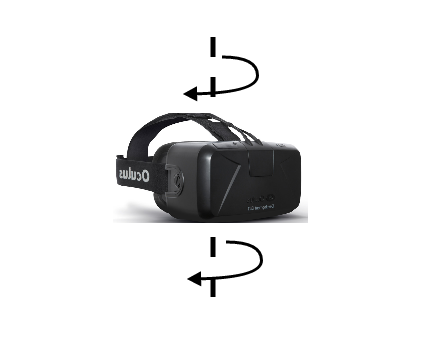
\includegraphics[width=60mm]{images/Robotrota.png}}
	\subfigure[La cámara gira respecto del eje X]{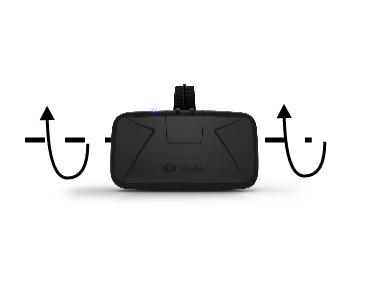
\includegraphics[width=60mm]{images/Robotexp.png}}\\
	\subfigure[Movimiento hacia delante si el ususario baja la cabeza]{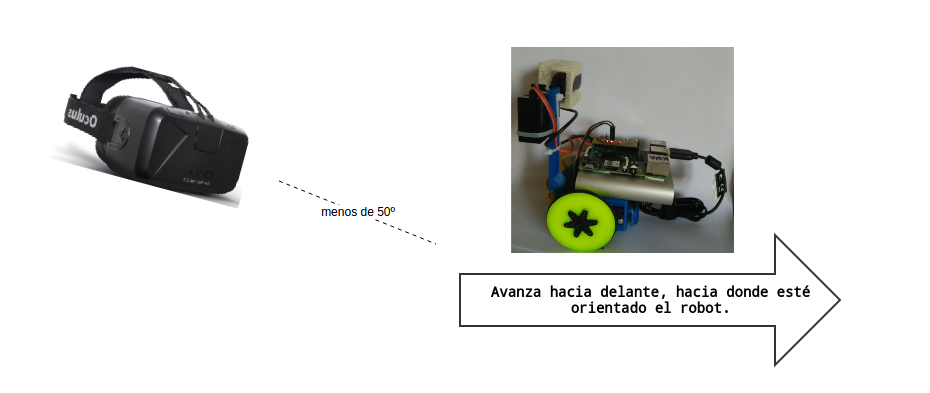
\includegraphics[width=120mm]{images/RobotAv.png}} %
	\caption{Posibles movimientos del robot según el movimiento de las Oculus Rift} \label{movRobot}
\end{figure}

Como viene explicado en la imagen \ref{movRobot}, si el usuario mira hacia los lados el robot rotará sobre sí mismo sin moverse del sitio, hacia la dirección que señalen las Oculus Rift.(\textbf{exploración})

Si el usuario mueve la cabeza hacia arriba o hacia abajo sin llegar a menos de 50º, la cámara se moverá como si fuera la cabeza del usuario.(\textbf{exploración})

En el caso de que el usuario oriente la cabeza hacia abajo, con un ángulo menor de 50º respecto al eje Y, la cámara se orientará horizontalmente (90º respecto al eje Y) y el robot avanzará hasta que el usuario cambie la posición de la cabeza.(\textbf{transporte})

\chapter{Pruebas y Resultados}

A continuación se explican las pruebas y los resultados obtenidos tras desarrollar el proyecto.

Puesto que el objetivo es crear un dispositivo sencillo de controlar por el usuario, las pruebas constarán de varias fases que se repetirán dentro de un ciclo cerrado. De esta forma el dispositivo podrá ir mejorando conforme a la demanda de los usuarios.

En la siguiente imagen se representan las diferentes fases del ciclo de pruebas.

\begin{figure}[h!]
	\centerline{
		\mbox{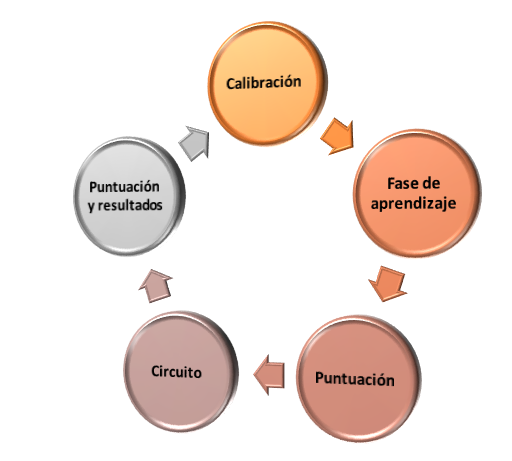
\includegraphics[width=.60\textwidth]{images/CicloPruebas.png}}
	}
	\caption{Fases del ciclo cerrado de pruebas que se han realizado para valorar la funcionalidad del dispositivo.}
\end{figure}

\section{Fases del ciclo cerrado}
\begin{itemize}
	\item \textbf{Calibración:} Ajustamos los parámetros de velocidad de los motores y sensibilidad de movimientos.
	\item \textbf{Fase de aprendizaje:} Se explica al usuario la interfaz y se deja que la pruebe durante un par de minutos.
	\item \textbf{Puntuación:}El usuario puntúa la interfaz y la facilidad de uso del dispositivo.
	\item \textbf{Circuito:} Se propone al usuario un circuito que debe seguir con el robot.
	\item \textbf{Puntuación y resultados:} Tras realizar el circuito e interaccionar con el dispositivo durante 5/10 minutos el usuario vuelve a puntuar y propone mejoras para la nueva fase de calibración.
\end{itemize}


\section{Desarrollo de las pruebas}
El primer ciclo se realizó con un único usuario ya que la interfaz aún no estaba claramente definida.

Tras este primer ciclo se realizaron dos ciclos más hasta que se consiguieron resultados satisfactorios.

A continuación se explicarán los resultados y mejoras realizadas en cada ciclo.

\subsection{Primer ciclo}

Como ya se ha explicado anteriormente, el primer ciclo de pruebas lo realizó un solo usuario ya que en base a sus valoraciones se modificó la interfaz prácticamente por completo.

\textbf{Antes de las pruebas} el robot se controlaba de la siguiente forma:
\begin{itemize}
	\item \textbf{Giros:} El robot giraba sobre sí mismo tantos grados como girara el usuario la cabeza.
	\item \textbf{Avanzar:} El robot avanzaba si el usuario mantenía la cabeza en posición natural, es decir, mirando hacia el frente.
	\item \textbf{Parar:} el robot se detenía cuando el usuario giraba la cabeza, es decir, en fase de exploración.
	\item \textbf{Movimiento de la cámara:} la cámara se movía tanto grados hacia arriba o hacia abajo como grados se moviera el usuario.
\end{itemize}

\paragraph{Valoración del usuario}
La primera valoración no fue muy positiva. A continuación se muestran las dificultades con las que se encontró el usuario:

\begin{itemize}
	\item [ - ] Giros: El usuario puso de manifiesto la dificultad que supone dar la vuelta al robot con la interfaz diseñada para este ciclo ya que el usuario tendría que girar sobre sí mismo.
	\subitem \textbf{Solución:} Modificar el giro de forma que el robot gire con velocidad continua hacia la derecha o izquierda según la orientación de la cabeza del usuario. 
	\item [ - ] Condición de parada: Otra dificultad con la que se encontró el usuario fue que la forma de parar el robot(girando la cabeza) era muy poco intuitiva.  A esto se le añade la dificultad de que el robot esté avanzando por defecto.
	\subitem \textbf{Solución:} Modificar el estado por defecto del dispositivo, en la nueva interfaz el robot está parado por defecto y en caso que esté en movimiento basta con mirar al frente para detenerlo.
\end{itemize}

Tras realizar las modificaciones da comienzo el segundo ciclo de pruebas.

\subsection{Segundo ciclo}

Durante el segundo ciclo de pruebas participaron 7 usuarios.
La fase de aprendizaje durante este ciclo consistió en:

\begin{itemize}
	\item Girar a la derecha
	\item Girar a la izquierda
	\item Mirar hacia arriba
	\item Estar 30 segundos aproximadamente girando el robot sobre sí mismo hasta tener controlado el giro.
	\item Andar hacia delante
	\item Parar
	\item Estar cerca de un minuto paseando para familiarizarse con los movimientos.
	\item Fijar un objetivo y alcanzarlo.
\end{itemize}

La siguiente tabla muestra la valoración de los usuarios tras realizar las pruebas.
\begin{center}
\begin{table}[h!]
\small
%\resizebox{15cm}{!} {

\begin{tabular}{|g  c  c  c  c  c  c  c |}
		\hline
	\rowcolor{yellow!50!white}           % Heading with different color to highlight it      
	\multicolumn{8}{|c|}{Valoración de los usuarios en el segundo ciclo} \\ \hline
	\rowcolor[gray]{0.8}
	& Usuario1 & Usuario2 & Usuario3 & Usuario4 & Usuario5 & Usuario6 & Usuario7\\
	 
	Giro derecha & 9 & 6 & 6 & 4 & 5 & 5 & 6\\
	Giro izquierda & 7.5 & 4 & 6 & 4 & 5 & 5 & 7\\
	Mirar hacia arriba & 9 & 10 & 9 & 10 & 9 & 9 & 9\\
	Andar & 10 & 8 & 10 & 8 & 8 & 9 & 9\\
	Parar & 9 & 10 & 9 & 7 & 7 & 7 & 8\\
	Alcanzar un objetivo & 8.5 & 6 & 8 & 7 & 5 & 5 & 8\\
	Sensación de Control & 7.5 & 6 & 9 & 4 & 5 & 4 & 7\\
	Facilidad de aprendizaje & 9 & 8 & 10 & 10 & 9 & 8 & 10\\
	\hline
\end{tabular}
\caption{Resultado de los test de usabilidad realizados por los usuarios al finalizar el segundo ciclo.}
%}
\end{table}
\end{center}

\paragraph{Comentarios tras las pruebas}

Analizando las puntuaciones y los comentarios de los usuarios se sacaron las siguientes conclusiones:

Se debe reducir la velocidad de giro ya que es complicado controlarlo a la velocidad actual.
La nueva interfaz de control del robot resulta mucho más intuitiva para los usuarios y su sensación de control incrementa en muy pocos minutos.

\subsection{Tercer ciclo}

A continuación se explicará el desarrollo del tercer y último ciclo de pruebas:
\begin{itemize}
	\item \textbf{Fase de calibración:} Durante esta fase se realizaron los siguientes cambios en base a la opinión de los usuarios que participaron en el segundo ciclo de pruebas:
	\begin{itemize}
		\item Se disminuyó la velocidad de giro de los servomotores de las ruedas del robot.
		\item Se disminuyó la velocidad de avance del robot.
		\item Se disminuyó la sensibilidad de detección de movimiento vertical , reduciendo las posibles posiciones que puede tomar la cámara a 4.
		\begin{itemize}
			\item Abajo: 30º aproximadamente respecto a la posición frontal.
			\item Posición frontal.
			\item Arriba: 40º aproximadamente respecto a la posición frontal.
			\item Arriba: 90º aproximadamente respecto a la posición frontal.
		\end{itemize}
	\end{itemize}
	\item \textbf{Fase de aprendizaje:} Se le explicó a cada usuario la forma de controlar el robot y se les dejó durante dos minutos moverse libremente.
	\item \textbf{Puntuación: } A continuación se muestra la primera puntuación de los usuarios.
	
\begin{center}

\begin{table}[h!]
\small	

	\begin{tabular}{|g c c c c c c|}
		\hline
		\rowcolor{yellow!50!white}           % Heading with different color to highlight it      
		\multicolumn{7}{|c|}{Valoración de los usuarios tras la fase de aprendizaje del tercer ciclo} \\ \hline
	\rowcolor[gray]{0.8}
		& Usuario1	&Usuario2	&Usuario3	&Usuario4	&Usuario5	&Usuario6 \\
		Avanzar
		 & 8 &7 &8 &9 &6 & 8\\
	Giro derecha
	 & 6 & 5 &6 &7 & 7& 6\\
		Giro izquierda
		 & 5 & 5&5 &5 &7 & 5\\
		Telepresencia
		 & 9 & 8 &8 & 7& 5& 6\\ 
		 Sensación de control
		 & 7 &4 &5 & 6&6 & 5\\
		 		 Interfaz
		 		 & 9 &7 & 7& 9& 6& 9\\
		 \hline
	\end{tabular}
	\caption{Resultado de los test de usabilidad realizados por los usuarios que participaron en el tercer ciclo de pruebas una vez finalizada la fase de aprendizaje}
\end{table}
\end{center}

\item \textbf{Circuito:} Los usuarios realizan el mismo circuito 3 veces. En el circuito se marcan 4 puntos críticos y se cronometra el tiempo que tarda cada usuario en alcanzar dichos puntos. También se cronometra el tiempo total.

A continuación se muestra un gráfico donde se muestran los promedios de tiempos entre todos los usuarios de cada intento de hacer el circuito.

\begin{figure}[h!]
	\centerline{
		\mbox{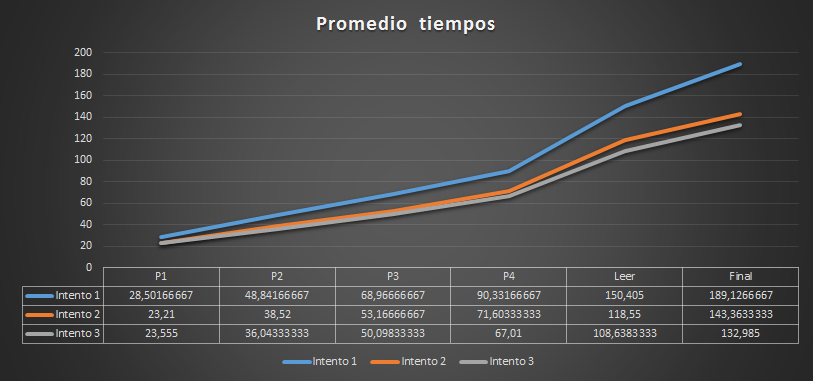
\includegraphics[width=.95\textwidth]{images/ResultadosTiempos.png}}
	}
	\caption{Promedio del tiempo que tardan los usuarios en realizar el circuito.}
\end{figure}
\item \textbf{Puntuación:} Por último se les vuelve a pedir a los usuarios que valoren el control del robot.

\begin{center}
\begin{table}[h!]
	\small

		\begin{tabular}{|g c c c c c c|}
			\hline
			\rowcolor{yellow!50!white}           % Heading with different color to highlight it      
			\multicolumn{7}{|c|}{Valoración de los usuarios tras realizar el circuito 3 veces} \\ \hline
			\rowcolor[gray]{0.8}
			& Usuario1	&Usuario2	&Usuario3	&Usuario4	&Usuario5	&Usuario6 \\
			Avanzar
			& 8 &9 &8 &6 &6 & 8\\
			Giro derecha
			& 7 & 7 &7 &8 & 6& 6\\
			Giro izquierda
			& 7 & 7&6 &8 &6 & 5\\
			Telepresencia
			& 9 & 8 &9 & 7& 6& 6\\ 
			Sensación de control
			& 8 &7 &7 & 6&7 & 5\\
			Interfaz
			& 9 &8 & 7& 9& 6& 9\\
			\hline
		\end{tabular}
		
		\caption{Resultado de los test de usabilidad realizados por los usuarios que participaron en el tercer ciclo de pruebas tras realizar el circuito}
	\end{table}
\end{center}

\newpage
Respecto a la valoración de los usuarios es muy interesante ver cómo varía la sensación de control que tienen los usuarios cuando empiezan a utilizar el dispositivo y cuando ya han realizado 3 veces el circuito. Dicha variaciónn se ve reflejada en el siguiente gráfico.

\begin{figure}[H]
	\centerline{
		\mbox{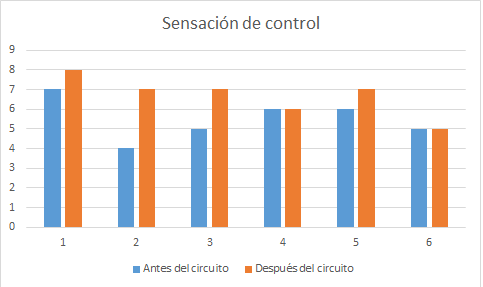
\includegraphics[width=.85\textwidth]{images/SensacionControl.png}}
	}
	\caption{Variación de la sensación de control de los usuarios antes y después de realizar el circuito.}
\end{figure}



\end{itemize}
%\section{Latencia de recepción de comandos}
%
%Para probar el sistema primero hemos hecho pruebas del funcionamiento de la red local, ya que en este trabajo es esencial tener poca latencia.
%
%Para ello se ha probado el alcance de la red inalámbrica, mandando comandos a los servomotores desde el ordeador.
%
%A continuación se ven los resultados obtenidos tras mandar comandos a una distancia de 7,5 metros y mandar comando estando el robot y el ordenador en habitaciones separadas
%
%\begin{figure}[h!]
%	\centerline{
%		\mbox{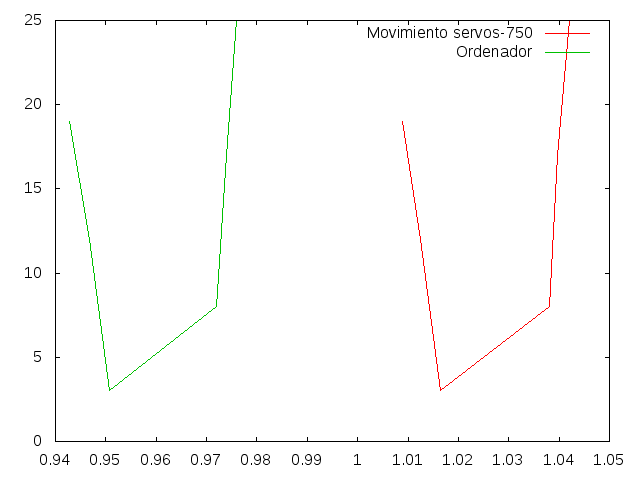
\includegraphics[width=.80\textwidth]{images/Temp_750.png}}
%	}
%	\caption{Diferencia de tiempos entre envío y recepción de comandos a 7,50 metros}
%\end{figure}
%
%\begin{figure}[h!]
%	\centerline{
%		\mbox{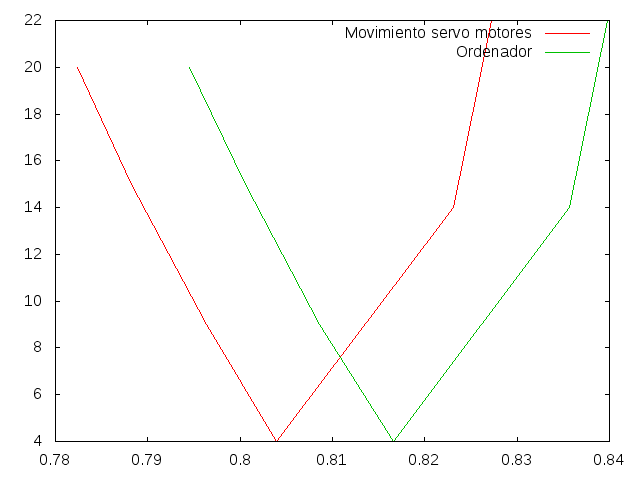
\includegraphics[width=.80\textwidth]{images/Temp_fuera.png}}
%	}
%	\caption{Diferencia de tiempos entre envío y recepción de comandos a 7,50 metros}
%\end{figure}
%
%Vemos que la latencia entre la medición en las Oculus y la recepción en la Raspberry es muy pequeña.
%
%En la gráfica que nos muestra la diferencia de tiempos a 7,5 metros vemos que de media el comando tarda en transmitirse menos de 0.5 segundos.
%
%En las pruebas entre habitaciones separadas, vemos que la diferencia no pasa de los 0,5 segundos por lo que creemos que es una latencia asumible ya que el robot no va a grandes velocidades.






\chapter{Conclusiones y trabajo futuro}
\label{chap:conclusiones}
\vspace{-0.2cm}

\section{Conclusiones}
En este apartado analizaremos los resultados obtenidos, hablaremos de posibles mejores y se expondrán las conclusiones del proyecto.

\paragraph{Puntos positivos y a mejorar}

Tras las pruebas se ve que el mayor defecto del proyecto es la \textbf{velocidad de giro} de los motores de las ruedas.

La calibración de servomotores es una tarea que se resuelve de forma experimental. La dificultad que nos encontramos es que la velocidad de giro cambia según en la superficie en la que se encuentre el robot por lo que habría que realizar las pruebas en diferentes entornos y hacer una calibración media.

Los usuarios han estado cada uno menos de 7 minutos con el robot y \textbf{todos menos uno lograron alcanzar su objetivo} en menos de un minuto, por lo que es una \textbf{aplicación fácil de manejar y de aprender}, como se ha visto en las valoraciones.

Otro problema es el \textbf{alcance de red de la Raspberry Pi 3}. Si el robot se alejaba mucho del router los servos seguín recibiendo correctamente los comandos pero el streaming tenía algo más de latencia.

Además la \textbf{Raspberry Pi 3 necesita de más amperaje que la Raspberry Pi 2} por lo que se concluye que por ahora, y hasta que se mejore la Raspberry Pi 3, es mejor utilizar Raspberry Pi 2 con un pincho Wifi para poder conectarse a la red local.

De esta forma se consigue mayor alcance de red y se necesita menos Amperios para alientar la placa.

A pesar de todos estos puntos a mejorar el resultado es muy bueno, teniendo e cuenta que e una primera aproximación a lo que que pretende ser un proyecto futuro.

Además es un proyecto con una \textbf{muy buena acogida}, a todos los usuarios les ha resultado ameno hacer las pruebas y ver cómo iban mejorando.

También es fácil de desarrollar con las herramientas de las que disponemos y con \textbf{mucho potencial}, ya que incluye dos tecnologías que están en pleno desarrollo y que aún tienen mucho que avanzar.

Otra ventaja es que hace uso de dispositivos de \textbf{fácil acceso} por lo que no resultaría demasiado caro de fabricar.

\subsection{Tecnologías aprendidas}

Durante la realización de este proyecto he utilizado muchas tecnologías, alguna de ellas completamente nuevas para mi.

El ejemplo más claro de esto son las gafas de realidad virtual Oculus Rift. Ha sido una suerte tener acceso a ellas y poder aprender a utilizar algunas de las librerías que hay disponibles para los desarrolladores.

También ha sido una sorpresa descubrir la gran variedad de posibilidades a desarrollar que permiten las Oculus, como es este proyecto.

He afianzado los conocimientos de robótica que ya tenía. Todo lo que sabía de robótica lo había aprendido en el Club de Robótica de esta universidad y gracias a este trabajo he podido aplicarlos y aumentarlos.

Todo el proyecto está desarrollado en python, lenguaje de programación que no he utilizado en ninguna asignatura de la carrera y que solo había visto muy por encima para proyectos sencillos.
Durante este proyecto he aprendido a utilizar la API de python disponible para las Oculus Rift y las librerías para el control de servomotores.

La placa base del robot es una Raspberry Pi 3, que tampoco había tenido la oportunidad de utilizarla nunca. De todas formas esto no ha sido novedoso para mi porque sí había participado en algún proyecto sencillo con Raspberry.

En conclusión este trabajo ha sido muy instructivo y ha ampliado de forma significativa mis conocimientos sobre robótica y realidad virtual.



\section{Trabajo futuro}
Este trabajo es solo el inicio de lo que podría ser un proyecto muy interesante.

El robot que hemos construido es una extensión del sentido de la vista, pero se podría construir un robot controlado por una persona y que fuera la extensión de todos sus sentidos,permitiendo así conocer y sentir el mundo sin necesidad de moverse de su casa.

Además la realidad virtual es una herramienta muy potente, que no solo te permite modificar tu mundo a placer sino que te premita crear entornos totalmente distintos. Se podría estudiar cómo interactuar con ese mundo virtual no solo a través de la vista , sino con todos los sentidos.

Otro camino por el que se puede investigar es la unión de este proyecto con la domótica.
Creo que en un futuro no muy lejano, las casas serán casas domotizadas, que igual que se podrán controlar desde el móvil podremos controlass con las gafas de realidad virtual.

\backmatter
\appendix

\cleardoublepage

\nocite{*}
\bibliography{hpcap40g}{}

\cleardoublepage
\printindex

\end{document}
